\documentclass{ws-ijait}

\graphicspath{{figures/}{figures/PoPS/}}

\usepackage{algpseudocode}
\usepackage{hyperref}
\usepackage{IEEEtrantools}
\usepackage{mathabx}
\usepackage{mathrsfs}
\usepackage{tikz}
\usetikzlibrary{shadows,patterns}

% BibTeX Packages
%\usepackage[super]{cite}
\usepackage{url}

\let\Problemheadfont\bfseries
\let\Problemfont\upshape
\newtheorem{problem}{Problem}

\let\Propertyheadfont\bfseries
\let\Propertyfont\upshape
\newtheorem{property}{Property}

\hypersetup{
  pdfauthor = {Nikolaos Pothitos and Panagiotis
               Stamatopoulos},
  pdftitle = {Building Search Methods with Self-confidence
              in a Constraint Programming Library},
  pdfsubject = {Computer Science, Artificial Intelligence},
  pdfkeywords = {randomness, stochastic methods,
                 discrepancy, constructive search, CSP}
}

\begin{document}

\markboth{Nikolaos Pothitos and Panagiotis Stamatopoulos}
         {Building Search Methods with Self-confidence in a
          Constraint Programming Library}

%%%%%%%%%%%%%%%%%%%%% Publisher's Area please ignore %%%%%%%%%%%%%%%
%
\catchline{}{}{}{}{}
%
%%%%%%%%%%%%%%%%%%%%%%%%%%%%%%%%%%%%%%%%%%%%%%%%%%%%%%%%%%%%%%%%%%%%

\title{Building Search Methods with Self-confidence in a \\
       Constraint Programming Library}

\author{Nikolaos Pothitos \and Panagiotis Stamatopoulos}

\address{Department of Informatics and Telecommunications \\
         National and Kapodistrian University of Athens \\
         Panepistimiopolis, 157\,84 Athens, Greece \\
         \{pothitos,takis\}@di.uoa.gr}

\maketitle

\begin{history}
  \received{(Day Month Year)}
  \revised{(Day Month Year)}
  \accepted{(Day Month Year)}
  %\comby{(xxxxxxxxxx)}
\end{history}

% Abstract should be less than 200 words
\begin{abstract}
  In the late 1990s, \emph{Constrained Programming} (CP)
  promised to separate the declaration of a problem from the
  process to solve it. This work attempts to serve this
  direction, by implementing and presenting a modular way to
  define \emph{search methods} that seek solutions to
  arbitrary \emph{Constraint Satisfaction Problems} (CSPs).
  The user just declares their CSP, and it can be solved
  using a portfolio of search methods already in place.
  Except from the pluggable search methods framework for any
  CSP, we also introduce pluggable \emph{heuristics} for our
  search methods. We found an efficient stochastic
  heuristics' paradigm that smoothly combines randomness
  with normal heuristics. We consider a factor of
  \emph{disobedience} to normal heuristics, and we fine-tune
  it each time, according to our estimation of normal
  heuristics' reliability (confidence). We prove
  mathematically that while the disobedience factor
  decreases, the stochastic heuristics approximate
  deterministic normal heuristics. Our algebraic evidence is
  supported by empirical evaluations on real life problems:
  A new search method, namely \textsc{PoPS}, that exploits
  this heuristics' paradigm, can outperform regular
  well-known constructive search methods.
\end{abstract}

\keywords{Randomness; stochastic methods; discrepancy;
          constructive search; CSP.}


\section{Introduction}

\emph{Artificial Intelligence} (AI) methodologies aim to
tackle with difficult computational and real life problems,
such as scheduling,\cite{Pinedo2012} radio frequency
assignment,\cite{Cabon1999} other NP-hard problems, and also
problems stemming from various disciplines, e.g.\ 
Bioinformatics.\cite{Barahona2011}

All these Constraint Satisfaction Problems or Constrained
Optimization Problems have been declared in our Constraint
Programming \textsc{Naxos Solver}.\cite{Naxos} In such
solvers, the solution phase is completely independent to the
CSP declaration phase, as this serves the original promise
of Constraint Programming: \emph{The user states the
problem, the computer solves it.}\cite{Freuder2014}

\subsection{Founding a search framework for Constraint
            Programming}

In this work, we go one step further and allow the
user\slash programmer to state their own \emph{search
methods} that can apply to any CSP. We found a framework
where the user can compose their search methods out of
conjunctive and disjunctive goals.

\textsc{Naxos Solver} is a C++ constraint programming
library. We implemented on top of it our search methods'
framework, but the framework can be adopted by other solvers
too. Our goal is not to compare \textsc{Naxos} against other
solvers, but to use it as an open source ground\slash
environment for this work's contributions.

Of course, Constraint Programming is not the only paradigm
that solves Artificial Intelligence problems like the
aforementioned. For example, course scheduling can be
addressed via plain simulated annealing.\cite{Zhang2010} In
comparison to Constraint Programming, this is not a complete
method, i.e.\ it doesn't explore all the possible solutions,
and therefore it doesn't always find the best solution, if
any.

Another way to solve the course scheduling problem is by
employing the simplex method in the context of linear
programming.\cite{Burke2010} In comparison to Constraint
Programming, linear programming is less expressive, as it
requires the formulation of every problem in a strict
mathematical model.\cite{Vanderbei2014}

\subsection{Stochastic heuristics revisited}

Naive search methods explore the whole candidate solutions
spectrum, in order to find a real solution. The issue here
is that the candidate solution range is exponential in the
problem instance parameters, and, unavoidably, an iteration
through every candidate solution becomes infeasible as the
problem scales.

\emph{Heuristics} role in this situation is to change the
order of the candidate solutions, so as to favor the
``promising'' ones. In other words, heuristics make an
estimation of the possibility of an incomplete or candidate
solution being a real solution, and label it with a
priority. A high priority means that the candidate solution
should be examined soon.

This reordering cannot make the search space
tractable---this is most probably
impossible\cite{Fortnow2009}---but it is able to
dramatically decrease the time needed to guide a search
method toward a real solution. In this direction, we study
heuristic properties, such as reliability\slash confidence,
and we propose a generic framework in order to exploit them
by incorporating a randomness factor into them. This work is
an extended and revised version of a preliminary conference
paper.\cite{Pothitos2016-PoPS}

In Section~\ref{preliminaries} we introduce just the
necessary formal definitions for CSPs. In
Section~\ref{search-framework} we found the framework that
can be used to define search methods; the algorithmic
details are isolated in \ref{framework-algorithm}. In
Section~\ref{search-tree} we explore a search tree by
consulting heuristics. In
Section~\ref{probabilistic-heuristics} we link heuristics
to probabilities and we bridge total determinism to total
randomness while consulting them. Section~\ref{PoPS}
illustrates a new search method, namely \textsc{PoPS}, that
exploits the values of the heuristic evaluations. Finally,
in Section~\ref{experiments} we conduct experiments to
support the previous theoretical sections.

In summary, the contributions of the paper are
\begin{itemize}
  \item the foundation of a modular \emph{search methods
        framework} for Constraint Programming,
  \item the introduction of a \emph{confidence} factor into
        regular heuristics and their gradual randomization
        when we aren't confident about them, in order to
        make them more flexible, and finally
  \item the implementation of an efficient \emph{new search
        method} \textsc{PoPS} that exploits heuristics as
        values\slash evaluations---as they are---and not
        simply as ranks of possible choices.
\end{itemize}


\section{Preliminaries\label{preliminaries}}

We focus on \emph{constraint satisfaction problems}
(CSPs)\cite{Tsang2014} that can be solved via a plethora of
available \emph{constraint programming} (CP)
solvers.\cite{ECLiPSe2017,Ilog2017}

\subsection{Constraint satisfaction problems}

Every single CSP can be stated using commonplace
formalizations.\cite{Russell2010} It is a triplet of
\begin{romanlist}
  \item \emph{constrained variables} $X_1, \ldots, X_n$,
  \item their corresponding \emph{domains} $D_{X_1}, \ldots,
        D_{X_n}$, which are normally finite sets of
        integers, and
  \item the \emph{constraints} between variables; a
        constraint contains the tuples of all the valid
        assignments for a specific pair\slash set of
        variables. To put it differently, a constraint is a
        relation between the variables, such as $X_1 < X_2$.
\end{romanlist}
In the attempt to find a solution to a CSP, we have to make
assignments.
\begin{definition}
  We say that a variable $X$ is \emph{assigned} a value $v
  \in D_X$, if its domain is made singleton, i.e.\ $D_X
  \leftsquigarrow \{v\}$.
\end{definition}
A \emph{solution} is an assignment that involves all
variables and also satisfies all the constraints. A
\emph{search method} leads a CSP after consecutive
assignments into a solution.

\subsection{Map-coloring problem}

There exists a huge list of interesting CSPs.\cite{Gent1999}
For example, \emph{map-coloring} is a CSP for assigning
colors to each prefecture in a given map, so as no
neighbouring prefectures have the same color.
Figure~\ref{map-colored} illustrates a map of the Greek
region ``Thessaly,'' containing four prefectures; the colors
in the figure form an indicative solution.

\begin{figure}
  \centering
  \input{figures/map-colored.pstex_t}
  \caption{The four Thessaly prefectures\label{map-colored}}
\end{figure}

\begin{problem}
  \label{thessaly-coloring}
  Typically, \emph{``Thessaly-coloring''} is a CSP with:
  \begin{romanlist}
    \item Four constrained variables: $X_1$, $X_2$, $X_3$,
          $X_4$. Each one of them contains the prefecture
          color.
    \item The corresponding domains are $D_{X_1} = D_{X_3} =
          \{1, 2\}$ and $D_{X_2} = D_{X_4} = \{1, 3\}$.
          Numbers \textcolor{red}{$1$}
          \textcolor{green}{$2$} \textcolor{blue}{$3$}
          represent respectively red, green,
          blue.\footnote{We could initially set all the
          domains equal to $\{1, 2, 3\}$. We used smaller
          initial domains just to simplify the problem.}
    \item The constraints are $X_1 \neq X_2$, $X_1 \neq
          X_3$, $X_2 \neq X_3$, and $X_2 \neq X_4$.
  \end{romanlist}
\end{problem}
The solution in Fig.~\ref{map-colored} is represented by the
assignment
\begin{equation}
  \label{solution}
  \{X_1 \gets \textcolor{red}{1}, \, X_2 \gets
  \textcolor{blue}{3}, \, X_3 \gets \textcolor{green}{2}, \,
  X_4 \gets \textcolor{red}{1}\} \, .
\end{equation}

\subsection{Constrained optimization\label{COP}}

A variation of Constraint Satisfaction Problems (CSPs) are
the so-called \emph{Constrained Optimization Problems}
(COPs). A COP consists of variables, domains, and
constraints, just like any CSP, but there are two
differences.
\begin{itemize}
  \item A COP also consists of an \emph{objective function}
        which maps any assignment\slash solution to a
        number, which is called the \emph{cost} of the
        solution.
  \item The target while solving a COP isn't just to find a
        solution, but to find a \emph{best} solution, i.e.\ 
        a solution with a minimum cost.
\end{itemize}
COPs can be solved like CSPs, using a \emph{branch and
bound} strategy: When a solution is found, its cost is
recorded, and a new constraint is added to guarantee that
the next solution cost will have a smaller cost than the
recorded one. This is repeated until all candidate solutions
have been examined.

In relation to CSP solving, the only additional requirement
of the above COP solving procedure is adding dynamically a
new constraint while searching. This makes it compatible
with plain CSP search methods, so this work covers both CSPs
and COPs as a whole.


\section{A Goal-driven Search Methods'
         Framework\label{search-framework}}

Except from a way to state CSPs, a user\slash programmer
needs an elegant way to state search methods that solve
them. The CSPs should be ``search-methods-agnostic,'' while
the search methods should be ``CSP-agnostic'' in order to
keep the independence between Constraint Programming stages.

In related works, a lot of search methods have been
implemented ``out of the box'' in modern
solvers.\cite{Gecode2017} This means, at least to our
knowledge, that the implemented search methods are coupled
with the existing solvers. Nevertheless, our contribution is
to introduce an extensible framework, so that the user can
easily define their own ``custom'' search methods.

\subsection{Search methods are made up of goals}

Every constructive search method is built up of goals. Each
goal executes an operation, e.g.\ an assignment of a value
to a constrained variable. Optionally, one goal returns
another goal to be executed. The goal returned can be a
\emph{meta}-goal, that is a goal that refers to another two
goals. There are two meta-goal kinds:
\begin{romanlist}
  \item The $\mathsf{AND}(g_1,g_2)$, which implies that the
        two sub-goals $g_1$ and $g_2$ must be executed and
        succeed both.
  \item The $\mathsf{OR}(g_1,g_2)$, which executes $g_1$. If
        $g_1$ does not succeed, i.e.\ if it does not lead to
        a solution, then $g_2$ is executed.
\end{romanlist}
This goal-driven framework is able to describe most of the
common search methods.

\subsection{The Depth-First Search example}

An elementary search method that can be straightforwardly
described via goals is \emph{depth-first search} (DFS). This
method iterates through the variables of a CSP\@. For each
variable $X$ selected, it selects a value $v$ from its
domain and makes the assignment $X \gets v$. It subsequently
proceeds to the next unassigned variable and makes another
assignment, etc.

If every variable is assigned a value and no constraint is
violated, the assignments set consists a \emph{solution}. In
any case, if there is a constraint violated, the last
assignment to a variable is undone and we try to assign
another value from its domain. If all the alternative values
are exhausted, we \emph{backtrack} to the previous variable
selected and we undo its assignment and so forth.

\subsection{Defining DFS using goals\label{DFS-goals}}

The ultimate goal in DFS and in every constructive search
method is to \texttt{Label} every variable with a value.
Each \texttt{Label}'s call aims to \texttt{Instantiate} a
variable.
\begin{itemize}
  \item \texttt{Label}($\emptyset$) := \textsf{success}.
  \item \texttt{Label}($\mathscr{X}$) :=
          \textsf{AND}(\texttt{Instantiate}($X$),
            \texttt{Label}($\mathscr{X} \! - \! \{X\}$)),
        with $X \in \mathscr{X}$,
\end{itemize}
where $\mathscr{X}$ is the set of all the variables. While
\texttt{Label} iterates recursively through the CSP
variables, an \texttt{Instantiate} call attempts to assign a
selected value $v$ to the variable $X$. If the assignment
fails to produce a solution, the value $v$ is deleted and
another instantiation is attempted, until all the
alternatives in $D_X$ are exhausted.
\begin{itemize}
  \item \texttt{Instantiate}($X$) := \textsf{failure},
          with $D_X = \emptyset$.
  \item \texttt{Instantiate}($X$) :=
          \textsf{OR}($X \! \gets \! v$,
            \textsf{AND}($D_X \!\! \gets \!\!
            D_X \!\! - \!\! \{v\}$,\,
            \texttt{Instantiate}($X$))), with $v \in D_X$.
\end{itemize}
The interdependencies between the above DFS goals are
graphically displayed in Fig.~\ref{DFS}.

\begin{figure}
  \centering
  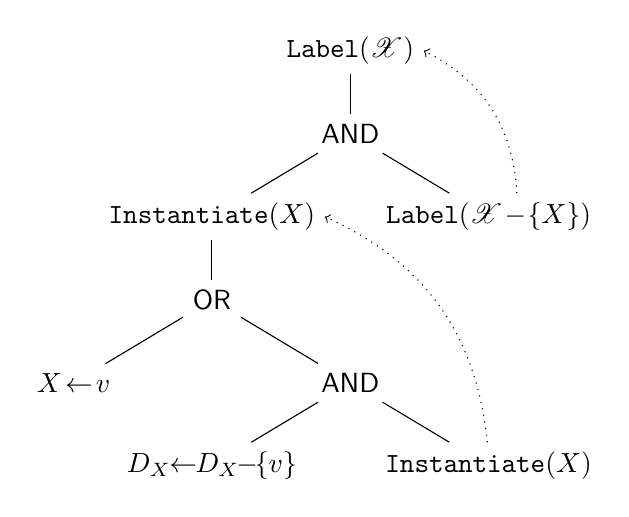
\begin{tikzpicture}
    [level distance = 3em, sibling distance = 10em,
     recursion/.style = {->, dotted, bend right}]
    \node (Label) {\texttt{Label}($\mathscr{X}$)}
      child {node {\textsf{AND}}
        child {node (Instantiate) {\texttt{Instantiate}($X$)}
          child {node {\textsf{OR}}
            child {node {$X \! \gets \! v$}}
            child {node {\textsf{AND}}
              child {node {$D_X \!\! \gets \!\! D_X \!\! - \!\! \{v\}$}}
              child {node (InstantiateChild) {\texttt{Instantiate}($X$)}}
            }
          }
        }
        child {node (LabelChild) {\texttt{Label}($\mathscr{X} \! - \! \{X\}$)}}
      };
    \path
      (LabelChild.40) edge [recursion] (Label.east)
      (InstantiateChild) edge [recursion] (Instantiate.east);
  \end{tikzpicture}
  \caption{The combination of the goals that compose
           DFS\label{DFS}}
\end{figure}

\begin{figure}
  \centering
  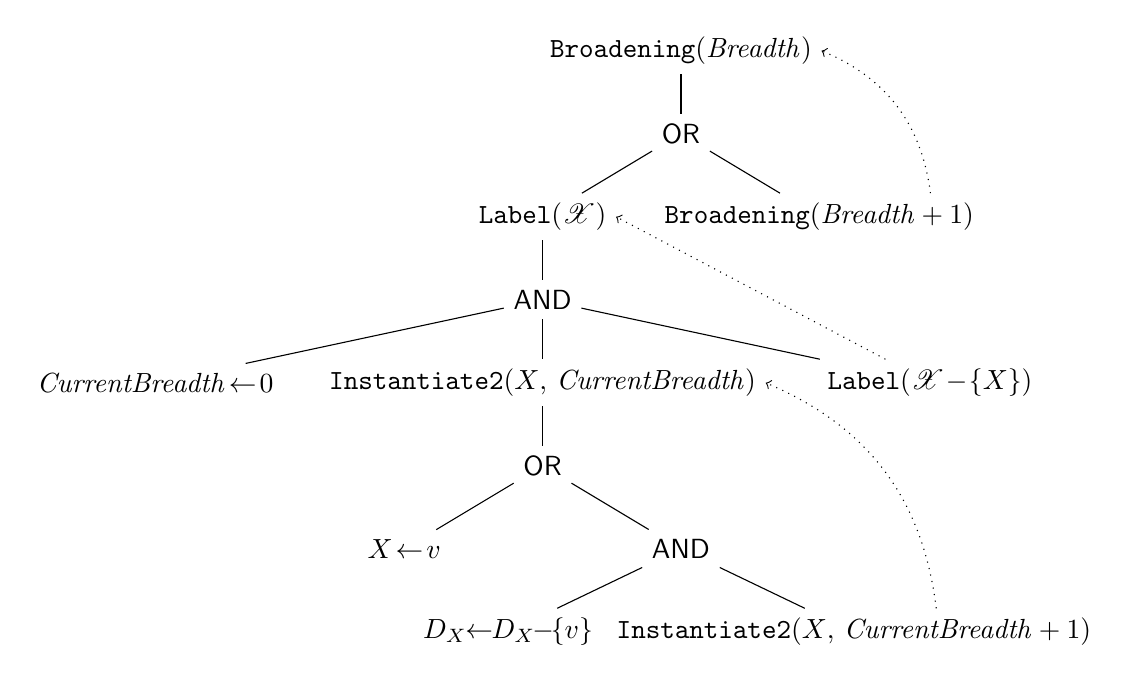
\begin{tikzpicture}
    [level distance = 3em, sibling distance = 10em,
     normalDistant/.style = {sibling distance = 10em},
     distant/.style = {sibling distance = 12.5em},
     moreDistant/.style = {sibling distance = 14em},
     recursion/.style = {->, dotted, bend right}]
    \node (Broadening) {\texttt{Broadening}($\mathit{Breadth}$)}
      child {node {\textsf{OR}}
        child {node (Label) {\texttt{Label}($\mathscr{X}$)}
          child {node {\textsf{AND}}
            child [moreDistant] {node {$\mathit{CurrentBreadth} \! \gets \! 0$}}
            child [moreDistant] {node (Instantiate) {\texttt{Instantiate2}($X$, $\mathit{CurrentBreadth}$)}
              child [normalDistant] {node {\textsf{OR}}
                child {node {$X \! \gets \! v$}}
                child {node {\textsf{AND}}
                  child [distant] {node {$D_X \!\! \gets \!\! D_X \!\! - \!\! \{v\}$}}
                  child [distant] {node (InstantiateChild) {\texttt{Instantiate2}($X$, $\mathit{CurrentBreadth} + 1$)}}
                }
              }
            }
            child [moreDistant] {node (LabelChild) {\texttt{Label}($\mathscr{X} \! - \! \{X\}$)}}
          }
        }
        child {node (BroadeningChild) {\texttt{Broadening}($\mathit{Breadth} + 1$)}}
      };
    \path
      (BroadeningChild.12) edge [recursion] (Broadening.east)
      (LabelChild) edge [->, dotted] (Label.east)
      (InstantiateChild.16) edge [recursion] (Instantiate.east);
  \end{tikzpicture}
  \caption{The goals composing Iterative
           Broadening\label{IBroadening}}
\end{figure}

\subsection{Defining Iterative Broadening using goals}

Figure~\ref{IBroadening} displays the corresponding goals'
graph for the \emph{Iterative Broadening} search
method.\cite{Ginsberg1992} The goals' structure is similar
to DFS. However, one basic difference is that there is one
more level, namely \texttt{Broadening}, above the ordinary
DFS goals.
\begin{itemize}
  \item \texttt{Broadening}($\mathit{Breadth}$) :=
          \textsf{failure}, if $\mathit{Breadth} > d$,
  \item \texttt{Broadening}($\mathit{Breadth}$) :=
          \textsf{AND}(\texttt{Label}($\mathscr{X}$),
            \texttt{Broadening}($\mathit{Breadth} + 1$)),
        otherwise.
\end{itemize}
For each Iterative Broadening iteration, the
$\mathit{Breadth}$ parameter defines the maximum number of
values that a constrained variable can be successively
assigned. This value is initially $1$. The
$\mathit{Breadth}$ value cannot exceed $d$, which in this
context is the maximum cardinality (size) of the domains of
all constrained variables. If $\mathit{Breadth}$ exceeds
$d$, \texttt{Broadening} fails.

Therefore, a second basic difference in comparison with DFS
comes into play. The \texttt{Instantiate} goal is now named
\texttt{Instantiate2}, and it takes one more argument.
\begin{itemize}
  \item \texttt{Instantiate2}($X$,
                              $\mathit{CurrentBreadth}$) :=
          \textsf{failure},
          if $D_X = \emptyset$,
  \item \texttt{Instantiate2}($X$,
                              $\mathit{CurrentBreadth}$) :=
          \textsf{failure},
          if $\mathit{CurrentBreadth} > \mathit{Breadth}$,
  \item \texttt{Instantiate2}($X$,
                              $\mathit{CurrentBreadth}$) :=
          \textsf{OR}($X \! \gets \! v$, \\
            \hspace*{\stretch{1}}
            \textsf{AND}($D_X \!\! \gets \!\!
                D_X \!\! - \!\! \{v\}$,\,
              \texttt{Instantiate2}($X$,
                $\mathit{CurrentBreadth} + 1$))), otherwise.
\end{itemize}
This implements Iterative Broadening's semantics: The number
of consecutive instantiations to the same variable cannot
exceed $\mathit{Breadth}$.


\section{Search Tree Exploration\label{search-tree}}

A \emph{search tree} is a descriptive way to depict every
possible assignment in a CSP, such as map-coloring.
Figure~\ref{pruned-tree} displays the search tree for the
Thessaly-coloring problem. The struck out nodes have been
pruned as no-goods.

\begin{figure}
  \centering
  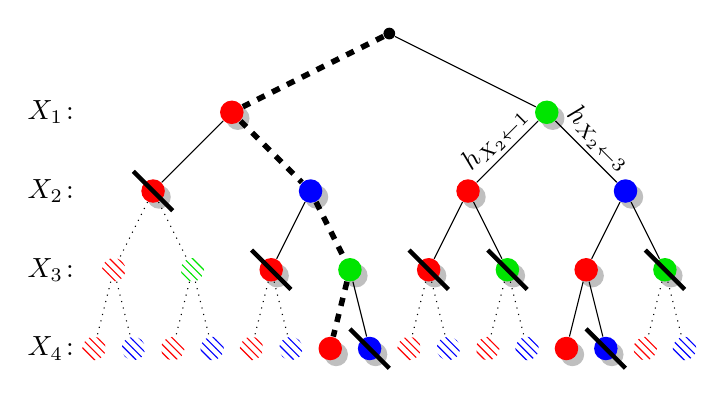
\begin{tikzpicture}
    [labelNode/.style = {inner sep = 0pt},
     rootNode/.style = {circle, fill, inner sep = 1.5pt},
     redNode/.style = {circle, fill, inner sep = 3pt, drop
                       shadow, red},
     greenNode/.style = {circle, fill, inner sep = 3pt, drop
                         shadow, green!90!black},
     blueNode/.style = {circle, fill, inner sep = 3pt, drop
                        shadow, blue},
     redPruned/.style = {circle, fill, inner sep = 3pt,
                         pattern = north west lines, pattern
                         color = red},
     greenPruned/.style = {circle, fill, inner sep = 3pt,
                           pattern = north west lines,
                           pattern color = green!90!black},
     bluePruned/.style = {circle, fill, inner sep = 3pt,
                          pattern = north west lines,
                          pattern color = blue},
     pruned/.style = {dotted},
     solution/.style = {line width = 2pt, dashed}]

    \node at (0,0) [rootNode] (root) {};

    \node at (-4.3,-1) [labelNode]   {$X_1 \! :$};
    \node at (-2,  -1) [redNode]     (R) {};
    \node at (+2,  -1) [greenNode]   (G) {};

    \node at (-4.3,-2) [labelNode] {$X_2 \! :$};
    \node at (-3,  -2) [redNode]     (RR) {};
      \draw [ultra thick] (-3.25,-1.75) -- (-2.75,-2.25);
    \node at (-1,  -2) [blueNode]    (RB) {};
    \node at (+1,  -2) [redNode]     (GR) {};
    \node at (+3,  -2) [blueNode]    (GB) {};

    \node at (-4.3,-3) [labelNode]   {$X_3 \! :$};
    \node at (-3.5,-3) [redPruned]   (RRR) {};
    \node at (-2.5,-3) [greenPruned] (RRG) {};
    \node at (-1.5,-3) [redNode]     (RBR) {};
      \draw [ultra thick] (-1.75,-2.75) -- (-1.25,-3.25);
    \node at (-0.5,-3) [greenNode]   (RBG) {};
    \node at (+0.5,-3) [redNode]     (GRR) {};
      \draw [ultra thick] (+0.25,-2.75) -- (+0.75,-3.25);
    \node at (+1.5,-3) [greenNode]   (GRG) {};
      \draw [ultra thick] (+1.25,-2.75) -- (+1.75,-3.25);
    \node at (+2.5,-3) [redNode]     (GBR) {};
    \node at (+3.5,-3) [greenNode]   (GBG) {};
      \draw [ultra thick] (+3.25,-2.75) -- (+3.75,-3.25);

    \node at (-4.3, -4) [labelNode]  {$X_4 \! :$};
    \node at (-3.75,-4) [redPruned]  (RRRR) {};
    \node at (-3.25,-4) [bluePruned] (RRRB) {};
    \node at (-2.75,-4) [redPruned]  (RRGR) {};
    \node at (-2.25,-4) [bluePruned] (RRGB) {};
    \node at (-1.75,-4) [redPruned]  (RBRR) {};
    \node at (-1.25,-4) [bluePruned] (RBRB) {};
    \node at (-0.75,-4) [redNode]    (RBGR) {};
    \node at (-0.25,-4) [blueNode]   (RBGB) {};
      \draw [ultra thick] (-0.5,-3.75) -- (0,-4.25);
    \node at (+0.25,-4) [redPruned]  (GRRR) {};
    \node at (+0.75,-4) [bluePruned] (GRRB) {};
    \node at (+1.25,-4) [redPruned]  (GRGR) {};
    \node at (+1.75,-4) [bluePruned] (GRGB) {};
    \node at (+2.25,-4) [redNode]    (GBRR) {};
    \node at (+2.75,-4) [blueNode]   (GBRB) {};
      \draw [ultra thick] (+2.5,-3.75) -- (+3,-4.25);
    \node at (+3.25,-4) [redPruned]  (GBGR) {};
    \node at (+3.75,-4) [bluePruned] (GBGB) {};

    \path
      (root) edge [solution] (R)
      (root) edge (G)

      (R) edge (RR)
      (R) edge [solution] (RB)
      (G) edge node [sloped, above = -2pt] {$h_{X_2 \gets 1}$} (GR)
      (G) edge node [sloped, above = -2pt] {$h_{X_2 \gets 3}$} (GB)

      (RR) edge [pruned] (RRR)
      (RR) edge [pruned] (RRG)
      (RB) edge (RBR)
      (RB) edge [solution] (RBG)
      (GR) edge (GRR)
      (GR) edge (GRG)
      (GB) edge (GBR)
      (GB) edge (GBG)

      (RRR) edge [pruned] (RRRR)
      (RRR) edge [pruned] (RRRB)
      (RRG) edge [pruned] (RRGR)
      (RRG) edge [pruned] (RRGB)
      (RBR) edge [pruned] (RBRR)
      (RBR) edge [pruned] (RBRB)
      (RBG) edge [solution] (RBGR)
      (RBG) edge (RBGB)
      (GRR) edge [pruned] (GRRR)
      (GRR) edge [pruned] (GRRB)
      (GRG) edge [pruned] (GRGR)
      (GRG) edge [pruned] (GRGB)
      (GBR) edge (GBRR)
      (GBR) edge (GBRB)
      (GBG) edge [pruned] (GBGR)
      (GBG) edge [pruned] (GBGB);
  \end{tikzpicture}
  \caption{The search tree for
           Thessaly-coloring\label{pruned-tree}}
\end{figure}

Each path from the root (i.e.\ the uppermost node)
represents an \emph{assignment}. If the path from the root
ends up into a leaf (lowest node), we have a \emph{complete}
assignment. E.g., the dotted path in Fig.~\ref{pruned-tree}
is an alternative form of the solution assignment in
\eqref{solution}.

\subsection{The goals are the search tree nodes}

There is a direct relationship between a search tree and the
goals hierarchy.
\begin{itemize}
  \item When the first goal, e.g.\ 
        \texttt{Label}($\mathscr{X}$) in DFS, is called, the
        search tree \emph{root} is created.
  \item When an \textsf{OR} goal occurs, the current node is
        extended into two branches that represent the two
        alternative choices.
\end{itemize}
In this work, we consider only sequential search methods.
Nevertheless, the presented search methods framework
naturally supports distributed search methods too. We can
simply distribute a search tree when we encounter an
\textsf{OR} goal. The left and right branches of selected
\textsf{OR} nodes can be explored concurrently to reduce the
total tree exploration time. There are many different
approaches regarding which \textsf{OR} nodes should be
selected in order to split their two
sub-trees.\cite{Regin2014,Pothitos2016-CPMR}

\subsection{Heuristic estimation as a real number}

A heuristic function maps every possible choice in the
search tree to a number that corresponds to the estimation
that it will eventually guide us toward a solution.
\begin{definition}
  \label{heuristic-function}
  For a specific search tree node, let $\mathsf{Choices}$ be
  the set with the alternative assignments that one may
  follow. The \emph{heuristic function} $h_i$ maps each
  alternative assignment $i \in \mathsf{Choices}$ to a
  positive number or zero, i.e.\ $h: \mathsf{Choices} \to
  \mathbb{R}^+$.
\end{definition}
\begin{example}
  \label{heuristic-function-example}
  In Fig.~\ref{pruned-tree} uppermost right node, there are
  two alternative assignments in $\mathsf{Choices} = \{X_2
  \gets 1, \, X_2 \gets 3\}$. One heuristic function may
  provide the estimations, e.g.\ $h_{X_2 \gets 1} = 0.7$ and
  $h_{X_2 \gets 3} = 2.8$; that is, the assignment $X_2
  \gets 3$ is more promising.
\end{example}
The above example is almost ideal, as the heuristic function
$h$ favours the assignment $X_2 \gets 3$ over $X_2 \gets 1$.
Besides, the latter leads to a dead end, as its two
descendants are struck out in Fig.~\ref{pruned-tree},
because they violate the constraints.

Unfortunately, this is not always the case, i.e.\ the
heuristic value for an assignment that leads to a dead end
(say $X_2 \gets 1$ in Fig.~\ref{pruned-tree}) may be
overestimated or, even worse, may be greater than the
heuristic estimation for an assignment that really leads to
a solution (e.g.\ $X_2 \gets 3$).

A heuristic value $h_i$ is actually a \emph{prediction}
whether a specific assignment will ultimately guide us to a
solution or not. Being a prediction, it implies an inherent
\emph{reliability\slash confidence} level.

In the above definition, we excluded negative values as the
heuristic function's output. A negative heuristic evaluation
could probably mean ``don't make this choice at all.'' But
heuristics are normally used to favour one choice over
another and not to prune a choice. In any case, if we had a
function $h$ with $\min h < 0$, we could transform it into
$h' = h + |\min h|$ to make it comply with the above
definition.

\subsection{Heuristics exploitation in related work}

In \emph{constructive search}, one can build a solution
either with a deterministic\slash systematic search method
or by making one-by-one random assignments. Do these methods
exploit heuristics and how?

\subsubsection{Deterministic search
               methods\label{deterministic}}

To our knowledge, existing search methods such as
\emph{limited discrepancy search} (LDS) use heuristics only
to \emph{order} the possible assignments and do not exploit
the \emph{difference} of the one heuristic estimation to
another, but only their \emph{rank}.\cite{Prosser2011} For
example, the \emph{iterative broadening} method explores
only a limited children's number for each search tree
node.\cite{Ginsberg1992} Of course, it chooses to visit only
the children with the highest ranks. \emph{Credit
search}\cite{Bartak2004} and \emph{limited assignment
number} (LAN)\cite{Bartak2005} are other deterministic
methods that also take into account the rank of the
heuristic estimations and not the heuristic values
themselves.

Last but not least, there are also methods that make the
assumption that \emph{the heuristic function is more
reliable as the search tree node depth increases.} E.g.,
\emph{depth-bounded discrepancy search} (DDS) allows to
override a heuristic estimation, only when we have not yet
reached a specific search tree depth.\cite{Walsh1997}
Finally, there are some methodologies that take into account
two or more heuristic functions and \emph{learn} as the
search proceeds, which heuristic is the best to
use.\cite{Xu2009}

\subsubsection{Random search methods\label{random}}

On the other hand, stochastic search methods completely
ignore heuristics, as they choose to make an assignment at
random.\cite{Jafari2011} For example, \emph{depth first
search with restarts} traverses the search tree making
random choices, and when a specific time limit is reached,
it re-starts from the beginning.

\subsubsection{Heuristics and probabilities}

Thus, the well-known search methods either use heuristics as
$\mathsf{Choices}$ ranks, or completely ignore them. In
1996, Bresina transformed the heuristic ranks into
\emph{probabilities} via the so-called
\emph{heuristic-biased stochastic sampling}
(HBSS).\cite{Bresina1996} He provided a set of various
decreasing functions $\mathsf{bias}(r)$, e.g.\ $\frac{1}{r}$
or $e^{-r}$ etc., that take a specific integer choice rank
$r \in \{1, 2, \ldots\}$ and return a number that
corresponds to the probability of the choice to be selected.
Cicirello and Smith improved HBSS by introducing the
\emph{value-biased stochastic sampling} (VBSS). The
$\mathsf{bias}$ function now takes as argument the heuristic
\emph{value} itself.\cite{Cicirello2005}

On the other hand, Gomes et al.\ exploit the so-called
\emph{heuristic-equivalence} to equate the choices with the
highest heuristic values.\cite{Gomes2000} In this way, we
can exclude the choices with the lower heuristic values and
select at random amongst the choices with the most
prevailing values.


\section{New Probabilistic
         Heuristics\label{probabilistic-heuristics}}

Our contribution lies in the mathematical foundation of a
framework that covers the above heuristic categories. In
contrast to existing methodologies, we leverage on the
\emph{smooth} transition from the total randomness to
determinism.

%\subsection{Heuristics linearization}
%
%In order to assign a probability to a specific choice, its
%heuristic estimation must be a real number. This is not
%always the case, because in general, heuristics are vectors
%of positive real numbers.
%\begin{definition}
%  A \emph{heuristic vector} $\mathbf{h} \in \mathbb{R}^n$
%  consists of multiple heuristic estimations. If $\mathbf{h}
%  = [h_{x_1} \; h_{x_2} \; \cdots \; h_{x_n}]$, the
%  $h_{x_1}$ is the \emph{primary heuristic estimation},
%  $h_{x_2}$ is the \emph{secondary heuristic estimation},
%  and $h_{x_n}$ is the \emph{$n$-ary heuristic estimation}
%  for the same choice.
%\end{definition}
%\begin{property}
%  A heuristic estimation $\mathbf{h_1}$ is stronger than
%  $\mathbf{h_2}$, iff $\mathbf{h_1}$ is lexicographically
%  greater than $\mathbf{h_2}$. In other words, the choice
%  $1$ that corresponds to $\mathbf{h_1}$ is preferable to
%  choice $2$, when $\mathbf{h_1} \succ_\mathrm{lex}
%  \mathbf{h_2}$.
%\end{property}
%\begin{example}
%  \label{vector}
%  Let $\mathbf{h_a} = [7 \; 4 \; 8]$, $\mathbf{h_b} = [2 \;
%  5 \; 3]$, and $\mathbf{h_c} = [7 \; 9 \; 6]$. Heuristic
%  $\mathbf{h_a}$ is stronger than $\mathbf{h_b}$, as it has
%  a greater primary heuristic estimation ($7 > 2$). However,
%  $\mathbf{h_a}$ is weaker than $\mathbf{h_c}$, as it has an
%  equal primary heuristic estimation ($7 = 7$), but a
%  smaller secondary ($4 < 9$).
%\end{example}
%An easy way to to make the vector $\mathbf{h}$ a simple real
%number, is to multiply each coordinate $h_{x_i}$ with a base
%$b_i$ and sum them all up.
%\begin{definition}
%  \label{linearization}
%  The \emph{linearization} of $\mathbf{h} = [h_{x_1} \;
%  h_{x_2} \; \cdots \; h_{x_n}]$ equals to $\mathsf{linear}
%  (\mathbf{h}) = h_{x_1} \cdot b_1 + h_{x_2} \cdot b_2 +
%  \cdots + h_{x_n} \cdot b_n$, where $b_n = 1$, $b_{n - 1} =
%  b_n \! \cdot \! ( \max h_{x_n} + 1 )$, \ldots, $b_1 = b_2
%  \! \cdot \! ( \max h_{x_2} + 1 )$.
%\end{definition}
%\begin{example}
%  Take the three vectors of Example~\ref{vector}. The
%  maximum secondary heuristic estimation is $\max h_{x_2} =
%  \max \{4, 5, 9\} = 9$. The maximum tertiary heuristic
%  estimation is $\max h_{x_3} = \max \{8, 3, 6\} = 8$.
%  Consequently, by applying Definition~\ref{linearization},
%  $b_3 = 1$, $b_2 = b_3 ( \max h_{x_3} + 1 ) = 1 (8 + 1) =
%  9$, and $b_1 = b_2 ( \max h_{x_2} + 1 ) = 9 (9 + 1) = 90$.
%
%  Thus, the linearizations of the vectors are
%  $\mathsf{linear} (\mathbf{h_a}) = 7 b_1 + 4 b_2 + 8 b_3 =
%  674$, $\mathsf{linear} (\mathbf{h_b}) = 2 b_1 + 5 b_2 + 3
%  b_3 = 228$, and $\mathsf{linear} (\mathbf{h_c}) = 7 b_1 +
%  9 b_2 + 6 b_3 = 717$.
%\end{example}
%\begin{proposition}
%  It can be proven that $\mathbf{h_1}$ is stronger than
%  $\mathbf{h_2}$, iff $\mathsf{linear} (\mathbf{h_1}) >
%  \mathsf{linear} (\mathbf{h_2})$.
%\end{proposition}
%Having transformed heuristic vectors into plain real
%numbers, we can now use them as probabilities.

\subsection{Heuristics probabilistic foundations}

Probabilities are a more precise way to depict heuristics
than orderings, because heuristics are actually
\emph{estimations} whether a choice will guide us to a
solution; they are not a strict quality rank.

\begin{definition}
  \label{hdf}
  A function $P: \mathsf{Choices} \to [0 \, , 1]\,,$ namely
  a \emph{heuristic distribution function}, maps each
  available choice to a corresponding probability, i.e.\ 
  $P(i)$.
\end{definition}
As in Definition~\ref{heuristic-function} and the
Example~\ref{heuristic-function-example} that follows it,
$\mathsf{Choices}$ may include all the possible\slash
candidate assignments to a constrained variable.
\begin{property}
  It should hold that $\sum_i P(i) = 1$, as $P$ denotes a
  probability for each $i \in \mathsf{Choices}$.
\end{property}
Regarding random search methods (Section~\ref{random}), the
probability is distributed uniformly along the
$\mathsf{Choices}$. Conclusively,
\begin{property}
  \label{probability-random}
  The heuristic distribution for a random method is always
  $P(i) = \frac{1}{|\mathsf{Choices}|}$, $\forall \, i$.
\end{property}
\begin{example}
  \label{distribution}
  Say that $\mathsf{Choices} = \{v_1, v_2, \ldots, v_5\}$.
  Every $v_i$ denotes a possible assignment. Furthermore, in
  a specific search tree node we can make five different
  assignments, and their corresponding heuristic estimations
  $h_i$ are $1$, $5$, $2$, $4$, $3$ respectively, as in
  Fig.~\ref{heuristics}.

  Figure~\ref{uniform} depicts the corresponding heuristic
  distribution function for a random method, that is $P(i) =
  \frac{1}{5}$, $\forall \, i$.
\end{example}

\begin{figure}
  \centering
  % GNUPLOT: LaTeX picture with Postscript
\begingroup
  \makeatletter
  \providecommand\color[2][]{%
    \GenericError{(gnuplot) \space\space\space\@spaces}{%
      Package color not loaded in conjunction with
      terminal option `colourtext'%
    }{See the gnuplot documentation for explanation.%
    }{Either use 'blacktext' in gnuplot or load the package
      color.sty in LaTeX.}%
    \renewcommand\color[2][]{}%
  }%
  \providecommand\includegraphics[2][]{%
    \GenericError{(gnuplot) \space\space\space\@spaces}{%
      Package graphicx or graphics not loaded%
    }{See the gnuplot documentation for explanation.%
    }{The gnuplot epslatex terminal needs graphicx.sty or graphics.sty.}%
    \renewcommand\includegraphics[2][]{}%
  }%
  \providecommand\rotatebox[2]{#2}%
  \@ifundefined{ifGPcolor}{%
    \newif\ifGPcolor
    \GPcolortrue
  }{}%
  \@ifundefined{ifGPblacktext}{%
    \newif\ifGPblacktext
    \GPblacktexttrue
  }{}%
  % define a \g@addto@macro without @ in the name:
  \let\gplgaddtomacro\g@addto@macro
  % define empty templates for all commands taking text:
  \gdef\gplbacktext{}%
  \gdef\gplfronttext{}%
  \makeatother
  \ifGPblacktext
    % no textcolor at all
    \def\colorrgb#1{}%
    \def\colorgray#1{}%
  \else
    % gray or color?
    \ifGPcolor
      \def\colorrgb#1{\color[rgb]{#1}}%
      \def\colorgray#1{\color[gray]{#1}}%
      \expandafter\def\csname LTw\endcsname{\color{white}}%
      \expandafter\def\csname LTb\endcsname{\color{black}}%
      \expandafter\def\csname LTa\endcsname{\color{black}}%
      \expandafter\def\csname LT0\endcsname{\color[rgb]{1,0,0}}%
      \expandafter\def\csname LT1\endcsname{\color[rgb]{0,1,0}}%
      \expandafter\def\csname LT2\endcsname{\color[rgb]{0,0,1}}%
      \expandafter\def\csname LT3\endcsname{\color[rgb]{1,0,1}}%
      \expandafter\def\csname LT4\endcsname{\color[rgb]{0,1,1}}%
      \expandafter\def\csname LT5\endcsname{\color[rgb]{1,1,0}}%
      \expandafter\def\csname LT6\endcsname{\color[rgb]{0,0,0}}%
      \expandafter\def\csname LT7\endcsname{\color[rgb]{1,0.3,0}}%
      \expandafter\def\csname LT8\endcsname{\color[rgb]{0.5,0.5,0.5}}%
    \else
      % gray
      \def\colorrgb#1{\color{black}}%
      \def\colorgray#1{\color[gray]{#1}}%
      \expandafter\def\csname LTw\endcsname{\color{white}}%
      \expandafter\def\csname LTb\endcsname{\color{black}}%
      \expandafter\def\csname LTa\endcsname{\color{black}}%
      \expandafter\def\csname LT0\endcsname{\color{black}}%
      \expandafter\def\csname LT1\endcsname{\color{black}}%
      \expandafter\def\csname LT2\endcsname{\color{black}}%
      \expandafter\def\csname LT3\endcsname{\color{black}}%
      \expandafter\def\csname LT4\endcsname{\color{black}}%
      \expandafter\def\csname LT5\endcsname{\color{black}}%
      \expandafter\def\csname LT6\endcsname{\color{black}}%
      \expandafter\def\csname LT7\endcsname{\color{black}}%
      \expandafter\def\csname LT8\endcsname{\color{black}}%
    \fi
  \fi
  \setlength{\unitlength}{0.0500bp}%
  \begin{picture}(4824.00,2016.00)%
    \gplgaddtomacro\gplbacktext{%
      \csname LTb\endcsname%
      \put(550,440){\makebox(0,0)[r]{\strut{}$\scriptstyle{0}$}}%
      \put(550,679){\makebox(0,0)[r]{\strut{}$\scriptstyle{1}$}}%
      \put(550,917){\makebox(0,0)[r]{\strut{}$\scriptstyle{2}$}}%
      \put(550,1156){\makebox(0,0)[r]{\strut{}$\scriptstyle{3}$}}%
      \put(550,1394){\makebox(0,0)[r]{\strut{}$\scriptstyle{4}$}}%
      \put(550,1633){\makebox(0,0)[r]{\strut{}$\scriptstyle{5}$}}%
      \put(1057,220){\makebox(0,0){\strut{}$v_1$}}%
      \put(1806,220){\makebox(0,0){\strut{}$v_2$}}%
      \put(2555,220){\makebox(0,0){\strut{}$v_3$}}%
      \put(3304,220){\makebox(0,0){\strut{}$v_4$}}%
      \put(4053,220){\makebox(0,0){\strut{}$v_5$}}%
      \put(176,1096){\rotatebox{-270}{\makebox(0,0){\strut{}$h_i$}}}%
    }%
    \gplgaddtomacro\gplfronttext{%
    }%
    \gplbacktext
    \put(0,0){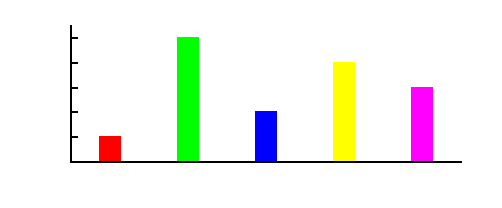
\includegraphics{heuristics}}%
    \gplfronttext
  \end{picture}%
\endgroup

  \caption{Heuristic estimations $h_i$ for each value
           $v_i$\label{heuristics}}
\end{figure}

\begin{figure}
  \centering
  % GNUPLOT: LaTeX picture with Postscript
\begingroup
  \makeatletter
  \providecommand\color[2][]{%
    \GenericError{(gnuplot) \space\space\space\@spaces}{%
      Package color not loaded in conjunction with
      terminal option `colourtext'%
    }{See the gnuplot documentation for explanation.%
    }{Either use 'blacktext' in gnuplot or load the package
      color.sty in LaTeX.}%
    \renewcommand\color[2][]{}%
  }%
  \providecommand\includegraphics[2][]{%
    \GenericError{(gnuplot) \space\space\space\@spaces}{%
      Package graphicx or graphics not loaded%
    }{See the gnuplot documentation for explanation.%
    }{The gnuplot epslatex terminal needs graphicx.sty or graphics.sty.}%
    \renewcommand\includegraphics[2][]{}%
  }%
  \providecommand\rotatebox[2]{#2}%
  \@ifundefined{ifGPcolor}{%
    \newif\ifGPcolor
    \GPcolortrue
  }{}%
  \@ifundefined{ifGPblacktext}{%
    \newif\ifGPblacktext
    \GPblacktexttrue
  }{}%
  % define a \g@addto@macro without @ in the name:
  \let\gplgaddtomacro\g@addto@macro
  % define empty templates for all commands taking text:
  \gdef\gplbacktext{}%
  \gdef\gplfronttext{}%
  \makeatother
  \ifGPblacktext
    % no textcolor at all
    \def\colorrgb#1{}%
    \def\colorgray#1{}%
  \else
    % gray or color?
    \ifGPcolor
      \def\colorrgb#1{\color[rgb]{#1}}%
      \def\colorgray#1{\color[gray]{#1}}%
      \expandafter\def\csname LTw\endcsname{\color{white}}%
      \expandafter\def\csname LTb\endcsname{\color{black}}%
      \expandafter\def\csname LTa\endcsname{\color{black}}%
      \expandafter\def\csname LT0\endcsname{\color[rgb]{1,0,0}}%
      \expandafter\def\csname LT1\endcsname{\color[rgb]{0,1,0}}%
      \expandafter\def\csname LT2\endcsname{\color[rgb]{0,0,1}}%
      \expandafter\def\csname LT3\endcsname{\color[rgb]{1,0,1}}%
      \expandafter\def\csname LT4\endcsname{\color[rgb]{0,1,1}}%
      \expandafter\def\csname LT5\endcsname{\color[rgb]{1,1,0}}%
      \expandafter\def\csname LT6\endcsname{\color[rgb]{0,0,0}}%
      \expandafter\def\csname LT7\endcsname{\color[rgb]{1,0.3,0}}%
      \expandafter\def\csname LT8\endcsname{\color[rgb]{0.5,0.5,0.5}}%
    \else
      % gray
      \def\colorrgb#1{\color{black}}%
      \def\colorgray#1{\color[gray]{#1}}%
      \expandafter\def\csname LTw\endcsname{\color{white}}%
      \expandafter\def\csname LTb\endcsname{\color{black}}%
      \expandafter\def\csname LTa\endcsname{\color{black}}%
      \expandafter\def\csname LT0\endcsname{\color{black}}%
      \expandafter\def\csname LT1\endcsname{\color{black}}%
      \expandafter\def\csname LT2\endcsname{\color{black}}%
      \expandafter\def\csname LT3\endcsname{\color{black}}%
      \expandafter\def\csname LT4\endcsname{\color{black}}%
      \expandafter\def\csname LT5\endcsname{\color{black}}%
      \expandafter\def\csname LT6\endcsname{\color{black}}%
      \expandafter\def\csname LT7\endcsname{\color{black}}%
      \expandafter\def\csname LT8\endcsname{\color{black}}%
    \fi
  \fi
  \setlength{\unitlength}{0.0500bp}%
  \begin{picture}(4824.00,2016.00)%
    \gplgaddtomacro\gplbacktext{%
      \csname LTb\endcsname%
      \put(726,440){\makebox(0,0)[r]{\strut{}$\scriptstyle{0}$}}%
      \put(726,679){\makebox(0,0)[r]{\strut{}$\scriptstyle{0.2}$}}%
      \put(726,917){\makebox(0,0)[r]{\strut{}$\scriptstyle{0.4}$}}%
      \put(726,1156){\makebox(0,0)[r]{\strut{}$\scriptstyle{0.6}$}}%
      \put(726,1394){\makebox(0,0)[r]{\strut{}$\scriptstyle{0.8}$}}%
      \put(726,1633){\makebox(0,0)[r]{\strut{}$\scriptstyle{1}$}}%
      \put(1215,220){\makebox(0,0){\strut{}$v_1$}}%
      \put(1929,220){\makebox(0,0){\strut{}$v_2$}}%
      \put(2642,220){\makebox(0,0){\strut{}$v_3$}}%
      \put(3356,220){\makebox(0,0){\strut{}$v_4$}}%
      \put(4070,220){\makebox(0,0){\strut{}$v_5$}}%
      \put(220,1096){\rotatebox{-270}{\makebox(0,0){\strut{}$P(i)$}}}%
    }%
    \gplgaddtomacro\gplfronttext{%
    }%
    \gplbacktext
    \put(0,0){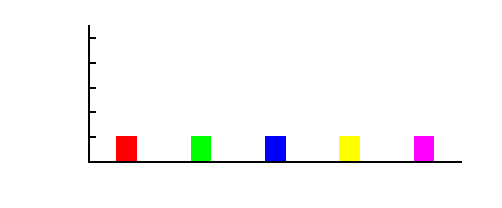
\includegraphics{uniform}}%
    \gplfronttext
  \end{picture}%
\endgroup

  \caption{The probability is spread
           uniformly\label{uniform}}
\end{figure}

\begin{figure}
  \centering
  % GNUPLOT: LaTeX picture with Postscript
\begingroup
  \makeatletter
  \providecommand\color[2][]{%
    \GenericError{(gnuplot) \space\space\space\@spaces}{%
      Package color not loaded in conjunction with
      terminal option `colourtext'%
    }{See the gnuplot documentation for explanation.%
    }{Either use 'blacktext' in gnuplot or load the package
      color.sty in LaTeX.}%
    \renewcommand\color[2][]{}%
  }%
  \providecommand\includegraphics[2][]{%
    \GenericError{(gnuplot) \space\space\space\@spaces}{%
      Package graphicx or graphics not loaded%
    }{See the gnuplot documentation for explanation.%
    }{The gnuplot epslatex terminal needs graphicx.sty or graphics.sty.}%
    \renewcommand\includegraphics[2][]{}%
  }%
  \providecommand\rotatebox[2]{#2}%
  \@ifundefined{ifGPcolor}{%
    \newif\ifGPcolor
    \GPcolortrue
  }{}%
  \@ifundefined{ifGPblacktext}{%
    \newif\ifGPblacktext
    \GPblacktexttrue
  }{}%
  % define a \g@addto@macro without @ in the name:
  \let\gplgaddtomacro\g@addto@macro
  % define empty templates for all commands taking text:
  \gdef\gplbacktext{}%
  \gdef\gplfronttext{}%
  \makeatother
  \ifGPblacktext
    % no textcolor at all
    \def\colorrgb#1{}%
    \def\colorgray#1{}%
  \else
    % gray or color?
    \ifGPcolor
      \def\colorrgb#1{\color[rgb]{#1}}%
      \def\colorgray#1{\color[gray]{#1}}%
      \expandafter\def\csname LTw\endcsname{\color{white}}%
      \expandafter\def\csname LTb\endcsname{\color{black}}%
      \expandafter\def\csname LTa\endcsname{\color{black}}%
      \expandafter\def\csname LT0\endcsname{\color[rgb]{1,0,0}}%
      \expandafter\def\csname LT1\endcsname{\color[rgb]{0,1,0}}%
      \expandafter\def\csname LT2\endcsname{\color[rgb]{0,0,1}}%
      \expandafter\def\csname LT3\endcsname{\color[rgb]{1,0,1}}%
      \expandafter\def\csname LT4\endcsname{\color[rgb]{0,1,1}}%
      \expandafter\def\csname LT5\endcsname{\color[rgb]{1,1,0}}%
      \expandafter\def\csname LT6\endcsname{\color[rgb]{0,0,0}}%
      \expandafter\def\csname LT7\endcsname{\color[rgb]{1,0.3,0}}%
      \expandafter\def\csname LT8\endcsname{\color[rgb]{0.5,0.5,0.5}}%
    \else
      % gray
      \def\colorrgb#1{\color{black}}%
      \def\colorgray#1{\color[gray]{#1}}%
      \expandafter\def\csname LTw\endcsname{\color{white}}%
      \expandafter\def\csname LTb\endcsname{\color{black}}%
      \expandafter\def\csname LTa\endcsname{\color{black}}%
      \expandafter\def\csname LT0\endcsname{\color{black}}%
      \expandafter\def\csname LT1\endcsname{\color{black}}%
      \expandafter\def\csname LT2\endcsname{\color{black}}%
      \expandafter\def\csname LT3\endcsname{\color{black}}%
      \expandafter\def\csname LT4\endcsname{\color{black}}%
      \expandafter\def\csname LT5\endcsname{\color{black}}%
      \expandafter\def\csname LT6\endcsname{\color{black}}%
      \expandafter\def\csname LT7\endcsname{\color{black}}%
      \expandafter\def\csname LT8\endcsname{\color{black}}%
    \fi
  \fi
  \setlength{\unitlength}{0.0500bp}%
  \begin{picture}(4824.00,2016.00)%
    \gplgaddtomacro\gplbacktext{%
      \csname LTb\endcsname%
      \put(726,440){\makebox(0,0)[r]{\strut{}$\scriptstyle{0}$}}%
      \put(726,679){\makebox(0,0)[r]{\strut{}$\scriptstyle{0.2}$}}%
      \put(726,917){\makebox(0,0)[r]{\strut{}$\scriptstyle{0.4}$}}%
      \put(726,1156){\makebox(0,0)[r]{\strut{}$\scriptstyle{0.6}$}}%
      \put(726,1394){\makebox(0,0)[r]{\strut{}$\scriptstyle{0.8}$}}%
      \put(726,1633){\makebox(0,0)[r]{\strut{}$\scriptstyle{1}$}}%
      \put(1215,220){\makebox(0,0){\strut{}$v_1$}}%
      \put(1929,220){\makebox(0,0){\strut{}$v_2$}}%
      \put(2642,220){\makebox(0,0){\strut{}$v_3$}}%
      \put(3356,220){\makebox(0,0){\strut{}$v_4$}}%
      \put(4070,220){\makebox(0,0){\strut{}$v_5$}}%
      \put(220,1096){\rotatebox{-270}{\makebox(0,0){\strut{}$P(i)$}}}%
    }%
    \gplgaddtomacro\gplfronttext{%
    }%
    \gplbacktext
    \put(0,0){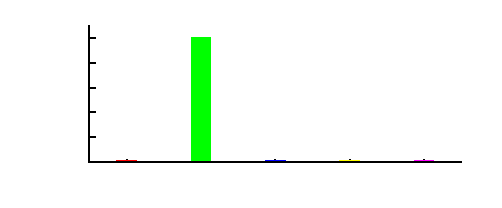
\includegraphics{systematic}}%
    \gplfronttext
  \end{picture}%
\endgroup

  \caption{Systematic search favours the highest
           $h_i$\label{systematic}}
\end{figure}

\begin{figure}
  \centering
  % GNUPLOT: LaTeX picture with Postscript
\begingroup
  \makeatletter
  \providecommand\color[2][]{%
    \GenericError{(gnuplot) \space\space\space\@spaces}{%
      Package color not loaded in conjunction with
      terminal option `colourtext'%
    }{See the gnuplot documentation for explanation.%
    }{Either use 'blacktext' in gnuplot or load the package
      color.sty in LaTeX.}%
    \renewcommand\color[2][]{}%
  }%
  \providecommand\includegraphics[2][]{%
    \GenericError{(gnuplot) \space\space\space\@spaces}{%
      Package graphicx or graphics not loaded%
    }{See the gnuplot documentation for explanation.%
    }{The gnuplot epslatex terminal needs graphicx.sty or graphics.sty.}%
    \renewcommand\includegraphics[2][]{}%
  }%
  \providecommand\rotatebox[2]{#2}%
  \@ifundefined{ifGPcolor}{%
    \newif\ifGPcolor
    \GPcolortrue
  }{}%
  \@ifundefined{ifGPblacktext}{%
    \newif\ifGPblacktext
    \GPblacktexttrue
  }{}%
  % define a \g@addto@macro without @ in the name:
  \let\gplgaddtomacro\g@addto@macro
  % define empty templates for all commands taking text:
  \gdef\gplbacktext{}%
  \gdef\gplfronttext{}%
  \makeatother
  \ifGPblacktext
    % no textcolor at all
    \def\colorrgb#1{}%
    \def\colorgray#1{}%
  \else
    % gray or color?
    \ifGPcolor
      \def\colorrgb#1{\color[rgb]{#1}}%
      \def\colorgray#1{\color[gray]{#1}}%
      \expandafter\def\csname LTw\endcsname{\color{white}}%
      \expandafter\def\csname LTb\endcsname{\color{black}}%
      \expandafter\def\csname LTa\endcsname{\color{black}}%
      \expandafter\def\csname LT0\endcsname{\color[rgb]{1,0,0}}%
      \expandafter\def\csname LT1\endcsname{\color[rgb]{0,1,0}}%
      \expandafter\def\csname LT2\endcsname{\color[rgb]{0,0,1}}%
      \expandafter\def\csname LT3\endcsname{\color[rgb]{1,0,1}}%
      \expandafter\def\csname LT4\endcsname{\color[rgb]{0,1,1}}%
      \expandafter\def\csname LT5\endcsname{\color[rgb]{1,1,0}}%
      \expandafter\def\csname LT6\endcsname{\color[rgb]{0,0,0}}%
      \expandafter\def\csname LT7\endcsname{\color[rgb]{1,0.3,0}}%
      \expandafter\def\csname LT8\endcsname{\color[rgb]{0.5,0.5,0.5}}%
    \else
      % gray
      \def\colorrgb#1{\color{black}}%
      \def\colorgray#1{\color[gray]{#1}}%
      \expandafter\def\csname LTw\endcsname{\color{white}}%
      \expandafter\def\csname LTb\endcsname{\color{black}}%
      \expandafter\def\csname LTa\endcsname{\color{black}}%
      \expandafter\def\csname LT0\endcsname{\color{black}}%
      \expandafter\def\csname LT1\endcsname{\color{black}}%
      \expandafter\def\csname LT2\endcsname{\color{black}}%
      \expandafter\def\csname LT3\endcsname{\color{black}}%
      \expandafter\def\csname LT4\endcsname{\color{black}}%
      \expandafter\def\csname LT5\endcsname{\color{black}}%
      \expandafter\def\csname LT6\endcsname{\color{black}}%
      \expandafter\def\csname LT7\endcsname{\color{black}}%
      \expandafter\def\csname LT8\endcsname{\color{black}}%
    \fi
  \fi
  \setlength{\unitlength}{0.0500bp}%
  \begin{picture}(4824.00,3376.80)%
    \gplgaddtomacro\gplbacktext{%
      \csname LTb\endcsname%
      \put(3466,711){\rotatebox{28}{\makebox(0,0)[l]{\strut{}$\mathsf{conf}$}}}%
    }%
    \gplgaddtomacro\gplfronttext{%
      \csname LTb\endcsname%
      \put(957,907){\makebox(0,0){\strut{}$v_1$}}%
      \put(1332,842){\makebox(0,0){\strut{}$v_2$}}%
      \put(1707,778){\makebox(0,0){\strut{}$v_3$}}%
      \put(2082,713){\makebox(0,0){\strut{}$v_4$}}%
      \put(2456,648){\makebox(0,0){\strut{}$v_5$}}%
      \put(2962,662){\makebox(0,0){\strut{}$\scriptstyle{0}$}}%
      \put(3200,785){\makebox(0,0){\strut{}$\scriptstyle{1}$}}%
      \put(3438,909){\makebox(0,0){\strut{}$\scriptstyle{2}$}}%
      \put(3676,1032){\makebox(0,0){\strut{}$\scriptstyle{3}$}}%
      \put(3915,1156){\makebox(0,0){\strut{}$\scriptstyle{4}$}}%
      \put(4153,1279){\makebox(0,0){\strut{}$\scriptstyle{5}$}}%
      \put(660,1051){\makebox(0,0)[r]{\strut{}$\scriptstyle{0}$}}%
      \put(660,1298){\makebox(0,0)[r]{\strut{}$\scriptstyle{0.2}$}}%
      \put(660,1545){\makebox(0,0)[r]{\strut{}$\scriptstyle{0.4}$}}%
      \put(660,1792){\makebox(0,0)[r]{\strut{}$\scriptstyle{0.6}$}}%
      \put(660,2037){\makebox(0,0)[r]{\strut{}$\scriptstyle{0.8}$}}%
      \put(660,2284){\makebox(0,0)[r]{\strut{}$\scriptstyle{1}$}}%
      \put(270,1757){\rotatebox{-270}{\makebox(0,0){\strut{}$P(i)$}}}%
    }%
    \gplbacktext
    \put(0,0){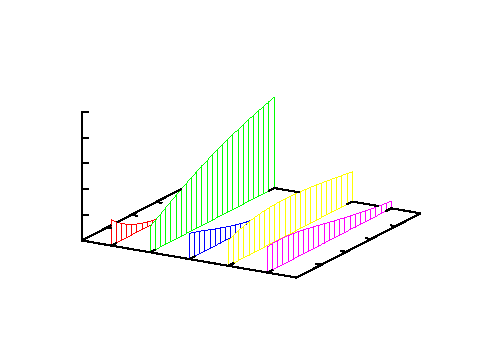
\includegraphics{conf}}%
    \gplfronttext
  \end{picture}%
\endgroup

  \caption{As $\mathsf{conf}$ rises, the effect to $P(i)$ is
           greater\label{conf}}
\end{figure}

On the other extreme, deterministic search methods
(Section~\ref{deterministic}) always select the choice $v_i$
that corresponds to the $h_i$ with the highest rank.
\begin{property}
  \label{probability-deterministic}
  Formally, in deterministic search methods, if $i =
  \arg\max_j h_j$, then $P(i) = 1$, otherwise $P(i) = 0$.
\end{property}
\begin{example}
  The greatest heuristic value in Example~\ref{distribution}
  is $h_2 = 5$. Hence, a deterministic search method would
  select $v_2$ with a certain probability $P(v_2) = 1$.
  Consequently, the rest of the probabilities are zero, as
  in Fig.~\ref{systematic}.
\end{example}
If there is more than one maximum heuristic value,
deterministic methods arbitrarily concern only one of them
as maximum. To simplify the following equations we will make
the assumption that there is only one maximum. Without loss
of generality, we also assume that heuristic values are
non-zero.

\subsection{Bridging the two opposites}

We extend our previous formulation of the heuristic
distribution function (Definition~\ref{hdf}) in order to
compromise random and deterministic methods. We introduce a
parameter $\mathsf{conf} \in \mathbb{R}^+$, that signifies
how much the heuristic estimations will be taken into
account; it is the heuristic's \emph{confidence}. This
$\mathsf{conf}$idence pararameter is the basis to define the
condition when a heuristic distribution function is
``balanced.''
\begin{definition}
  \label{balanced}
  A parameterized heuristic distribution function
  $P_\mathsf{conf} (i)$ is \emph{balanced} if and only if:
  \begin{enumerate}
    \item[1.] $\forall \, i$, ${\displaystyle
              \lim_{\mathsf{conf} \to 0} } \!\!
              P_\mathsf{conf} (i) =
              \frac{1}{|\mathsf{Choices}|}$, and
    \item[2a.] if $i = \arg\max_j h_j$, ${\displaystyle
               \lim_{\mathsf{conf} \to \infty} } \!\!\!\!
               P_\mathsf{conf} (i) = 1$,
    \item[2b.] otherwise, ${\displaystyle
               \lim_{\mathsf{conf} \to \infty} } \!\!\!\!
               P_\mathsf{conf} (i) = 0 \,$.
  \end{enumerate}
  Moreover, the function $P_\mathsf{conf} (i)$ must be
  monotonic and continuous with respect to $\mathsf{conf}$
  and for fixed $i$.
\end{definition}
Intuitively, $\mathsf{conf}$ is the link between random and
deterministic search methods, as the above definition covers
both Property~\ref{probability-random} when $\mathsf{conf}
\to 0$ and Property~\ref{probability-deterministic} when
$\mathsf{conf} \to \infty$. In other words, $\mathsf{conf}$
is the position along the random-deterministic axis.

What happens for intermediate $\mathsf{conf}$ values? This
depends on the precise parameterized heuristic distribution
function instance. We define the following function that
gradually scales randomness.
\begin{lemma}
  \label{exponential}
  The function $P_\mathsf{conf} (i) =
  \frac{h_i^\mathsf{conf}}{\sum_j h_j^\mathsf{conf}}$ is
  balanced.\footnote{For $\mathsf{conf} = 1$, the function
  $P_1 (i) = \frac{h_i}{\sum_j h_j}$ is equivalent to the
  \emph{fitness proportionate selection}
  function---resembling a \emph{roulette wheel}---that is
  used in Genetic Algorithms.\cite{Sharma2012}}
\end{lemma}
\begin{proof}
  We prove Definition~\ref{balanced} three requirements.
  \begin{enumerate}
    \item[1.] ${\displaystyle \lim_{\mathsf{conf} \to 0} }
              \!\! P_\mathsf{conf} (i) =
              \frac{h_i^0}{\sum\limits_{j \in
              \mathsf{Choices}} \!\!\!\! h_j^0} =
              \frac{1}{\sum\limits_{j \in \mathsf{Choices}}
              \!\!\!\!\! 1} = \frac{1}{|\mathsf{Choices}|}
              \, $.
              \vspace{0.3em}
    \item[2a.] Let $n = |\mathsf{Choices}|$. This number is
               bounded as the possible assignments in a CSP
               are a finite set. Thus, the distribution
               function can be analyzed as
               \[
                 P_\mathsf{conf} (i) = {\textstyle
                 \frac{h_i^\mathsf{conf}}{\sum_j
                 h_j^\mathsf{conf}} } = {\textstyle
                 \frac{h_i^\mathsf{conf}}{h_1^\mathsf{conf}
                 + h_2^\mathsf{conf} + \cdots +
                 h_{\max}^\mathsf{conf} + \cdots +
                 h_n^\mathsf{conf}} } \, .
               \]
               Let $h_{\max}$ be the maximum $h_i$. If we
               divide by $h_{\max}^\mathsf{conf}$ both the
               nominator and denominator, we have
               \begin{IEEEeqnarray}{rCl}
                 P_\mathsf{conf} (i)
                 & = &
                 {\textstyle
                  \frac{\left(\frac{h_i}{h_{\max}}\right)^\mathsf{conf}}{\left(\frac{h_1}{h_{\max}}\right)^\mathsf{conf}
                  + \cdots + 1 + \cdots +
                  \left(\frac{h_n}{h_{\max}}\right)^\mathsf{conf}}
                 } \nonumber \\
                 & = &
                 {\textstyle
                  \frac{\left(\frac{h_i}{h_{\max}}\right)^\mathsf{conf}}{1
                  + \sum_{j \neq \max}
                  \left(\frac{h_j}{h_{\max}}\right)^\mathsf{conf}}
                 } \, . \label{function}
               \end{IEEEeqnarray}
               Here, $\max$ is an abbreviation for
               $\arg\max_i h_i$. Therefore, $\forall \, j
               \neq \max$,
               \begin{IEEEeqnarray}{rCl}
                 h_j < h_{\max} & \  \Rightarrow \  &
                 \frac{h_j}{h_{\max}} < 1
                 \  \Rightarrow \  \nonumber \\
                 & & \!\!\! {\displaystyle
                 \lim_{\mathsf{conf} \to \infty}}
                 \left(\frac{h_j}{h_{\max}}\right)^\mathsf{conf}
                 \!\!\! = 0 \, . \quad
                 \label{limit}
               \end{IEEEeqnarray}
               As a result from \eqref{function} and
               \eqref{limit},
               \begin{IEEEeqnarray}{rCl}
                 \lim_{\mathsf{conf} \to \infty} \!\!\!\!
                 P_\mathsf{conf} (i)
                 & = &
                 {\textstyle \frac{\lim_{\mathsf{conf} \to
                  \infty}
                  \left(\frac{h_i}{h_{\max}}\right)^\mathsf{conf}}{1
                  + \sum_{j \neq \max} \lim_{\mathsf{conf}
                  \to \infty}
                  \left(\frac{h_j}{h_{\max}}\right)^\mathsf{conf}}
                 } \nonumber \\
                 & = &
                 \lim_{\mathsf{conf} \to \infty} {\textstyle
                 \left(\frac{h_i}{h_{\max}}\right)^\mathsf{conf}
                 } .
                 \label{final-limit}
               \end{IEEEeqnarray}
               A direct derivation is that for $i = \max
               \equiv \arg\max_j h_j$, we have
               $\lim_{\mathsf{conf} \to \infty}
               P_\mathsf{conf} (\max) = 1$, which is the
               second prerequisite for a balanced function.
               \vspace{0.3em}
    \item[2b.] Finally, the last prerequisite of
               Definition~\ref{balanced} involves $i \neq
               \max \Rightarrow h_i < h_{\max} \Rightarrow
               \frac{h_i}{h_{\max}} < 1$, which, combined
               with \eqref{final-limit}, gives
               $\lim_{\mathsf{conf} \to \infty}
               P_\mathsf{conf} (i) = 0$, which had to be
               demonstrated.
  \end{enumerate}
\end{proof}
The above function (in Lemma~\ref{exponential}) is balanced,
and it also moves smoothly from the random extreme to the
deterministic one, because it is a \emph{continuous}
function, with regard to $\mathsf{conf} \in \mathbb{R}^+$.

Hence, the overall function is a transition from the total
randomness to the almost total determinism. This is
illustrated in the three-dimensional Fig.~\ref{conf}, which
for $\mathsf{conf} = 0$, is equivalent to the
two-dimensional Fig.~\ref{uniform}, and when $\mathsf{conf}
\to \infty$, it is equivalent to Fig.~\ref{systematic}.

Furthermore, our initial goal was to propose flexible
heuristics which perform better than purely deterministic or
purely stochastic ones. To implement and measure the
transition from randomness to determinism, we just
introduced a \emph{confidence} value. However, new questions
now arise. Which $\mathsf{conf}$ value should be used? Which
is the best way to bind the proposed hybrid heuristics to
search processes?


\section{Piece of Pie Search\label{PoPS}}

The probabilistic framework founded in the previous section,
naturally complies with existing search methods; it affects
only the heuristic function and not the methods themselves.
But in order to fully exploit the introduced heuristics
framework, we built the new constructive search method
\emph{Piece of Pie Search} (\textsc{PoPS}).

\subsection{The algorithm's core}

Figure~\ref{PopsSample} describes \textsc{PopsSample}, which
is the \textsc{PoPS} core. It is called inside \textsc{PoPS}
in order to solve a CSP by providing a complete and valid
$\mathsf{Assignments}$ set, which is initially empty.

\begin{figure}
  \centering
  \begin{algorithmic}
    \Function{PopsSample}{$\mathsf{PieceToCover}, \mathsf{conf}$}
      \State \textbf{local variables:}
      \State \quad $\mathsf{Assignments}$: set with all the
             assignments made until this call
      \State \quad $\mathscr{X}$: set with all the
             constrained variables
      \State \quad $X$: constrained variable that is going
             to be instantiated
      \State \quad $\mathsf{value}$: value that is going to
             be assigned
      \State \quad $h_{X \gets v}$: heuristic value for the
             assignment $X \gets v$
      \State \quad $D_{X_\mathrm{init}}$: initial domain of
             $X$, before any assignment was made
      \State \quad $D_X$: current domain of $X$
      \State \quad $\mathit{CoveredPiece}$: current covered
             proportion of the pie
      \State
      \If {$\mathsf{Assignments}$ violate any constraint}
        \State \Return failure
      \ElsIf {$\mathsf{Assignments}$ include every variable}
        \State Record $\mathsf{Assignments}$ as solution
        \State \Return success
      \EndIf
      \State $X \, \gets \,
              \Call{VariablesOrderHeuristic}{\mathscr{X}}$
      \State $D_{X_\mathrm{init}} \, \gets \, D_X$
      \State $\mathit{CoveredPiece} \, \gets \, 0$
      \While {$\mathit{CoveredPiece} \, \leq \,
               \mathsf{PieceToCover}$}
        \State $\mathsf{value} \, \gets \,
                \Call{ValuesOrderHeuristic}{D_X, \mathsf{conf}}$
        \State $\mathit{CoveredPiece} \, \gets \,
                \mathit{CoveredPiece} \, + \,
                \frac{h_{X \gets \mathsf{value}}^\mathsf{conf}}
                     {\sum_{v \in D_{X_\mathrm{init}}}
                      h_{X \gets v}^\mathsf{conf}}$
        \State Assign $\mathsf{value}$ to $X$ and add it to
               $\mathsf{Assignments}$
        \State \Call{PopsSample}{$\mathsf{PieceToCover}, \,
                     \mathsf{conf} \! + \!
                     \frac{100 - \mathsf{conf}}{|\mathscr{X}|}$}
        \State Undo the assignment
        \State $D_X \, \gets \, D_X - \{\mathsf{value}\}$
      \EndWhile
      \State $D_X \, \gets \, D_{X_\mathrm{init}}$
        \Comment{Restores initial domain}
      \State \Return failure
        \Comment{All alternative values are exhausted}
    \EndFunction
  \end{algorithmic}
  \caption{The recursive {\normalfont\textsc{PopsSample}}
           called by
           {\normalfont\textsc{PoPS}}\label{PopsSample}}
\end{figure}

In each \textsc{PopsSample} call we get an unassigned
variable returned by the function
\textsc{VariablesOrderHeuristic}($\mathscr{X}$), where
$\mathscr{X}$ is the set of all the constrained variables.
Then, it stores its domain $D_X$, in order to restore it in
a future backtrack. All the above steps are common in
constructive search methods.

The crucial and novel part of this function is inside the
\textbf{while} iteration where we iterate through the
different values in $D_X$. The call
\textsc{ValuesOrderHeuristic}($D_X, \mathsf{conf}$) returns
the best value out of $D_X$, according to the heuristic
estimation, using the heuristic function in
Lemma~\ref{exponential}.

Normal search methods, like Depth First Search (DFS),
Limited Discrepancy Search (LDS), and other known
deterministic methods explore in their steps a specific
\emph{number} of values in $D_X$ or every value in it (cf.\ 
Section~\ref{deterministic}). In \textsc{PopsSample}, we
explore a specific \emph{subset} $D_X'$ of $D_X$, which
corresponds to a proportion of the heuristics pie. The
proportion is the argument $\mathsf{PieceToCover} \in
[0,1]$. When $\mathsf{PieceToCover}$ is $1$,
\textsc{PopsSample} becomes a complete search method as it
explores all the $D_X$ set values.
\begin{example}
  \label{heuristics-pie}
  Figure~\ref{piechart} demonstrates the
  heuristics-probabilities pie for the
  Example~\ref{distribution}: Each $P(i)$ corresponds to a
  value $v_i$ in $D_X$. In this case, a
  \textsc{PopsSample}($0.5, 1$) invocation would explore
  half the pie. E.g., the choices that correspond to the
  heuristics $P(1) + P(2) + P(3)$ or $P(2) + P(5)$ make half
  the pie and more.

  A more detailed step by step explanation follows.
  \begin{itemize}
    \item We are inside the \textbf{while} loop of a
          \textsc{PopsSample}($0.5, 1$) call.
    \item $\mathit{CoveredPiece}$ is initially $0$; the loop
          stops when $\mathit{CoveredPiece}$ exceeds $0.5$.
    \item \textsc{ValuesOrderHeuristic}($D_X, 1$) is called.
    \item According to Example~\ref{distribution}, this
          function will return a value out of $\{v_1, v_2,
          v_3, v_4, v_5\}$.
    \item Each value $v_i$ has been evaluated with an
          heuristic value $h_i$.
    \item Most specifically, $h_1 = 1$, $h_2 = 5$, $h_3 =
          2$, $h_4 = 4$, and $h_5 = 3$.
    \item The probability that $v_i$ is selected by
          \textsc{ValuesOrderHeuristic} is $P(i)$, which is
          calculated using the above evaluations together
          with Lemma~\ref{exponential}.
    \item Thus, the respective probabilities are $P(1) =
          0.07$, $P(2) = 0.33$, $P(3) = 0.13$, $P(4) =
          0.27$, and $P(5) = 0.20$.
    \item Again, all the above are \emph{probabilities}
          ($P(i)$) of the event that a specific value
          ($v_i$) will be selected. Therefore, every value
          can be selected in each iteration.
    \item Suppose that $v_5$ is selected at the first
          iteration with $P(5) = 0.20$.
    \item This probability is also used to increase the
          current $\mathit{CoveredPiece}$, which becomes
          $0.20$ too.
    \item $X$ is assigned $v_5$.
  \end{itemize}
  After the assignment, \textsc{PopsSample}($0.5, 1 +
  \frac{99}{|\mathscr{X}|}$) is called. Please note the
  slight incease of the $\mathsf{conf}$ value. This
  recursive call will choose another variable out of
  $\mathscr{X}$ and enter the \textbf{while} loop again.
  This loop will try to assign a value to the new variable
  from its domain. If the attempts fail, we continue back to
  the first \textbf{while} loop, which was described in the
  above bullets.
  \begin{itemize}
    \item The assignment of $v_5$ to $X$ is undone, $v_5$ is
          removed from the domain, and another iteration
          begins.
    \item We proceed to the second iteration, as the
          $\mathsf{PieceToCover}$ ($0.5$) is still greater
          than the $\mathit{CoveredPiece}$ ($0.2$).
    \item Let's say that $v_2$ is then chosen by
          \textsc{ValuesOrderHeuristic} with a $P(2) = 0.33$
          probability.
    \item $\mathit{CoveredPiece}$ now equals $0.20 + 0.33 =
          0.53$.
  \end{itemize}
  Again, \textsc{PopsSample}($0.5, 1 +
  \frac{99}{|\mathscr{X}|}$) is called. If the attempts to
  instantiate the next variable fail, we are back to the
  first \textbf{while} loop:
  \begin{itemize}
    \item The assignment of $v_2$ to $X$ is undone.
    \item We proceed to the third iteration.
    \item However, $\mathit{CoveredPiece}$ ($0.53$) is now
          greater than $\mathsf{PieceToCover}$ ($0.5$).
    \item More than half of the pie of the choices for $X$
          has been already explored; no other alternatives
          are examined.
    \item The rest of the values $v_1$, $v_3$, $v_4$ are
          left unused\slash unexplored. This makes
          \textsc{PopsSample} an \emph{incomplete} search
          method, as it may override a solution (which
          involves for example these values) for the sake of
          speed.
  \end{itemize}
\end{example}

Again, LDS is an incomplete search method too; at each
search tree node it may explore only a limited \emph{number}
of the available choices. The difference with our method is
that we may explore a limited \emph{proportion} of the
heuristics pie of choices, which makes our method more
``heuristics-aware.'' This means that the number of the
explored choices by our method in a specific node may vary,
depending on how the heuristics pie is distributed to the
choices. On the other hand, LDS explores a fixed number of
choices, independently of the heuristics pie distribution.

It's worth noting that while more variables get
instantiated, the $\mathsf{conf}$ value gradually increases.
Besides, heuristic estimations tend to be more reliable when
we have less unassigned variables.

\begin{figure}
  \centering
  % GNUPLOT: LaTeX picture with Postscript
\begingroup
  \makeatletter
  \providecommand\color[2][]{%
    \GenericError{(gnuplot) \space\space\space\@spaces}{%
      Package color not loaded in conjunction with
      terminal option `colourtext'%
    }{See the gnuplot documentation for explanation.%
    }{Either use 'blacktext' in gnuplot or load the package
      color.sty in LaTeX.}%
    \renewcommand\color[2][]{}%
  }%
  \providecommand\includegraphics[2][]{%
    \GenericError{(gnuplot) \space\space\space\@spaces}{%
      Package graphicx or graphics not loaded%
    }{See the gnuplot documentation for explanation.%
    }{The gnuplot epslatex terminal needs graphicx.sty or graphics.sty.}%
    \renewcommand\includegraphics[2][]{}%
  }%
  \providecommand\rotatebox[2]{#2}%
  \@ifundefined{ifGPcolor}{%
    \newif\ifGPcolor
    \GPcolortrue
  }{}%
  \@ifundefined{ifGPblacktext}{%
    \newif\ifGPblacktext
    \GPblacktexttrue
  }{}%
  % define a \g@addto@macro without @ in the name:
  \let\gplgaddtomacro\g@addto@macro
  % define empty templates for all commands taking text:
  \gdef\gplbacktext{}%
  \gdef\gplfronttext{}%
  \makeatother
  \ifGPblacktext
    % no textcolor at all
    \def\colorrgb#1{}%
    \def\colorgray#1{}%
  \else
    % gray or color?
    \ifGPcolor
      \def\colorrgb#1{\color[rgb]{#1}}%
      \def\colorgray#1{\color[gray]{#1}}%
      \expandafter\def\csname LTw\endcsname{\color{white}}%
      \expandafter\def\csname LTb\endcsname{\color{black}}%
      \expandafter\def\csname LTa\endcsname{\color{black}}%
      \expandafter\def\csname LT0\endcsname{\color[rgb]{1,0,0}}%
      \expandafter\def\csname LT1\endcsname{\color[rgb]{0,1,0}}%
      \expandafter\def\csname LT2\endcsname{\color[rgb]{0,0,1}}%
      \expandafter\def\csname LT3\endcsname{\color[rgb]{1,0,1}}%
      \expandafter\def\csname LT4\endcsname{\color[rgb]{0,1,1}}%
      \expandafter\def\csname LT5\endcsname{\color[rgb]{1,1,0}}%
      \expandafter\def\csname LT6\endcsname{\color[rgb]{0,0,0}}%
      \expandafter\def\csname LT7\endcsname{\color[rgb]{1,0.3,0}}%
      \expandafter\def\csname LT8\endcsname{\color[rgb]{0.5,0.5,0.5}}%
    \else
      % gray
      \def\colorrgb#1{\color{black}}%
      \def\colorgray#1{\color[gray]{#1}}%
      \expandafter\def\csname LTw\endcsname{\color{white}}%
      \expandafter\def\csname LTb\endcsname{\color{black}}%
      \expandafter\def\csname LTa\endcsname{\color{black}}%
      \expandafter\def\csname LT0\endcsname{\color{black}}%
      \expandafter\def\csname LT1\endcsname{\color{black}}%
      \expandafter\def\csname LT2\endcsname{\color{black}}%
      \expandafter\def\csname LT3\endcsname{\color{black}}%
      \expandafter\def\csname LT4\endcsname{\color{black}}%
      \expandafter\def\csname LT5\endcsname{\color{black}}%
      \expandafter\def\csname LT6\endcsname{\color{black}}%
      \expandafter\def\csname LT7\endcsname{\color{black}}%
      \expandafter\def\csname LT8\endcsname{\color{black}}%
    \fi
  \fi
  \setlength{\unitlength}{0.0500bp}%
  \begin{picture}(3810.96,3376.80)%
    \gplgaddtomacro\gplbacktext{%
      \csname LTb\endcsname%
      \put(3276,1804){\makebox(0,0){\strut{}$P(1)$}}%
      \put(2057,2867){\makebox(0,0){\strut{}$P(2)$}}%
      \put(534,1804){\makebox(0,0){\strut{}$P(3)$}}%
      \put(1202,346){\makebox(0,0){\strut{}$P(4)$}}%
      \put(3041,719){\makebox(0,0){\strut{}$P(5)$}}%
    }%
    \gplgaddtomacro\gplfronttext{%
    }%
    \gplbacktext
    \put(0,0){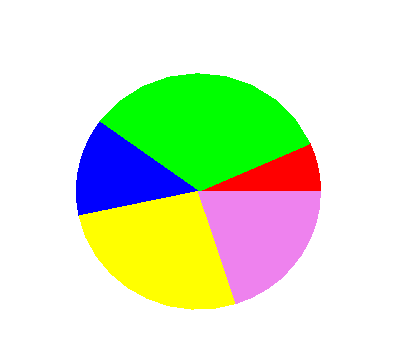
\includegraphics{piechart}}%
    \gplfronttext
  \end{picture}%
\endgroup

  \caption{The heuristics-probabilities pie chart for
           Example~\ref{distribution}\label{piechart}}
\end{figure}

\begin{example}
  \label{heuristics-pie2}
  We will consider the above Example~\ref{heuristics-pie}
  for a \textsc{PopsSample}($0.5, 2$) call, i.e.\ for
  $\mathsf{conf} = 2$.

  According to Lemma~\ref{exponential}, the probalilities
  for $\mathsf{conf} = 2$ are computed as $P_2(i) =
  \frac{h_i^2}{\sum_j h_j^2}$. For example, $P_2(1) =
  \frac{h_1^2}{\sum_j h_j^2} = \frac{1^2}{1^2 + 5^2 + 2^2 +
  4^2 + 3^2} = 0.02$. The other probabilities are $P_2(2) =
  0.45$, $P_2(3) = 0.07$, $P_2(4) = 0.29$, and $P_2(5) =
  0.16$. Thus, the pie is redistributed as in
  Figure~\ref{piechart2}.

  While $\mathsf{conf}$-idence increases, the value $v_2$
  which had initially the greatest heuristic evaluation
  $h_2$ is even more likely to be selected, as $P(2)$
  increases too. In other words, we get closer to total
  determinism and closer to complete confidence in the
  highest heuristic evaluation: In total determinism (in
  systematic search) $v_2$ would have been always selected
  with a certain probability $1$.
\end{example}

\begin{figure}
  \centering
  % GNUPLOT: LaTeX picture with Postscript
\begingroup
  \makeatletter
  \providecommand\color[2][]{%
    \GenericError{(gnuplot) \space\space\space\@spaces}{%
      Package color not loaded in conjunction with
      terminal option `colourtext'%
    }{See the gnuplot documentation for explanation.%
    }{Either use 'blacktext' in gnuplot or load the package
      color.sty in LaTeX.}%
    \renewcommand\color[2][]{}%
  }%
  \providecommand\includegraphics[2][]{%
    \GenericError{(gnuplot) \space\space\space\@spaces}{%
      Package graphicx or graphics not loaded%
    }{See the gnuplot documentation for explanation.%
    }{The gnuplot epslatex terminal needs graphicx.sty or graphics.sty.}%
    \renewcommand\includegraphics[2][]{}%
  }%
  \providecommand\rotatebox[2]{#2}%
  \@ifundefined{ifGPcolor}{%
    \newif\ifGPcolor
    \GPcolortrue
  }{}%
  \@ifundefined{ifGPblacktext}{%
    \newif\ifGPblacktext
    \GPblacktexttrue
  }{}%
  % define a \g@addto@macro without @ in the name:
  \let\gplgaddtomacro\g@addto@macro
  % define empty templates for all commands taking text:
  \gdef\gplbacktext{}%
  \gdef\gplfronttext{}%
  \makeatother
  \ifGPblacktext
    % no textcolor at all
    \def\colorrgb#1{}%
    \def\colorgray#1{}%
  \else
    % gray or color?
    \ifGPcolor
      \def\colorrgb#1{\color[rgb]{#1}}%
      \def\colorgray#1{\color[gray]{#1}}%
      \expandafter\def\csname LTw\endcsname{\color{white}}%
      \expandafter\def\csname LTb\endcsname{\color{black}}%
      \expandafter\def\csname LTa\endcsname{\color{black}}%
      \expandafter\def\csname LT0\endcsname{\color[rgb]{1,0,0}}%
      \expandafter\def\csname LT1\endcsname{\color[rgb]{0,1,0}}%
      \expandafter\def\csname LT2\endcsname{\color[rgb]{0,0,1}}%
      \expandafter\def\csname LT3\endcsname{\color[rgb]{1,0,1}}%
      \expandafter\def\csname LT4\endcsname{\color[rgb]{0,1,1}}%
      \expandafter\def\csname LT5\endcsname{\color[rgb]{1,1,0}}%
      \expandafter\def\csname LT6\endcsname{\color[rgb]{0,0,0}}%
      \expandafter\def\csname LT7\endcsname{\color[rgb]{1,0.3,0}}%
      \expandafter\def\csname LT8\endcsname{\color[rgb]{0.5,0.5,0.5}}%
    \else
      % gray
      \def\colorrgb#1{\color{black}}%
      \def\colorgray#1{\color[gray]{#1}}%
      \expandafter\def\csname LTw\endcsname{\color{white}}%
      \expandafter\def\csname LTb\endcsname{\color{black}}%
      \expandafter\def\csname LTa\endcsname{\color{black}}%
      \expandafter\def\csname LT0\endcsname{\color{black}}%
      \expandafter\def\csname LT1\endcsname{\color{black}}%
      \expandafter\def\csname LT2\endcsname{\color{black}}%
      \expandafter\def\csname LT3\endcsname{\color{black}}%
      \expandafter\def\csname LT4\endcsname{\color{black}}%
      \expandafter\def\csname LT5\endcsname{\color{black}}%
      \expandafter\def\csname LT6\endcsname{\color{black}}%
      \expandafter\def\csname LT7\endcsname{\color{black}}%
      \expandafter\def\csname LT8\endcsname{\color{black}}%
    \fi
  \fi
  \setlength{\unitlength}{0.0500bp}%
  \begin{picture}(3810.96,3376.80)%
    \gplgaddtomacro\gplbacktext{%
      \csname LTb\endcsname%
      \put(3311,1612){\makebox(0,0){\strut{}$P_2(1)$}}%
      \put(1928,2879){\makebox(0,0){\strut{}$P_2(2)$}}%
      \put(499,1432){\makebox(0,0){\strut{}$P_2(3)$}}%
      \put(1402,256){\makebox(0,0){\strut{}$P_2(4)$}}%
      \put(3135,867){\makebox(0,0){\strut{}$P_2(5)$}}%
    }%
    \gplgaddtomacro\gplfronttext{%
    }%
    \gplbacktext
    \put(0,0){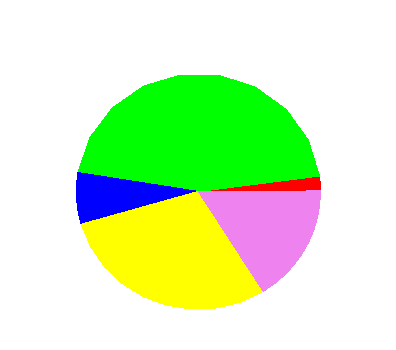
\includegraphics{piechart2}}%
    \gplfronttext
  \end{picture}%
\endgroup

  \caption{The previous heuristics-probabilities pie chart
           when $\mathsf{conf} = 2$\label{piechart2}}
\end{figure}

\newcommand{\PoPS}{\textbf{\normalsize P\footnotesize
                           O\normalsize PS}}
\newcommand{\PopsSample}{\textbf{\normalsize P\footnotesize
                       OPS\normalsize S\footnotesize AMPLE}}

\subsection{\PopsSample{} declaration using our search
            methods framework}

Figure~\ref{PopsSampleGoals} expresses graphically the
\textsc{PopsSample} method using our search methods
framework (Section~\ref{search-framework}).

\begin{figure}
  \centering
  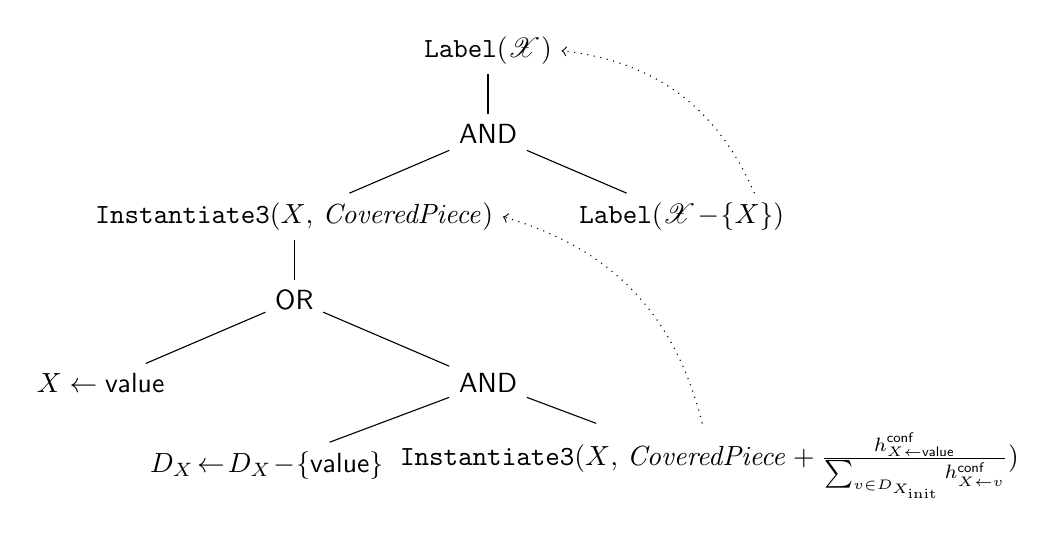
\begin{tikzpicture}
    [level distance = 3em, sibling distance = 12em,
     distant/.style = {sibling distance = 14em},
     moreDistant/.style = {sibling distance = 16em},
     recursion/.style = {->, dotted, bend right}]
    \node (Label) {\texttt{Label}($\mathscr{X}$)}
      child {node {\textsf{AND}}
        child [distant] {node (Instantiate) {\texttt{Instantiate3}($X$, $\mathit{CoveredPiece}$)}
          child {node {\textsf{OR}}
            child {node {$X \gets \mathsf{value}$}}
            child {node {\textsf{AND}}
              child [moreDistant] {node {$D_X \! \gets \! D_X \! - \! \{\mathsf{value}\}$}}
              child [moreDistant] {node (InstantiateChild) {\texttt{Instantiate3}($X$, $\mathit{CoveredPiece} + \frac{h_{X \gets \mathsf{value}}^\mathsf{conf}} {\sum_{v \in D_{X_\mathrm{init}}} h_{X \gets v}^\mathsf{conf}}$)}}
            }
          }
        }
        child [distant] {node (LabelChild) {\texttt{Label}($\mathscr{X} \! - \! \{X\}$)}}
      };
    \path
      (LabelChild.18) edge [recursion] (Label.east)
      (InstantiateChild) edge [recursion] (Instantiate.east);
  \end{tikzpicture}
  \caption{The goals that build up
           \textsc{PopsSample}\label{PopsSampleGoals}}
\end{figure}

One essential difference with DFS is the instantiation goal
for each variable. \texttt{Instantiate3} takes one more
argument, namely $\mathit{CoveredPiece}$. When this exceeds
$\mathsf{PieceToCover}$, the goal fails.
\begin{itemize}
  \item \texttt{Instantiate3}($X$,
                              $\mathit{CoveredPiece}$) :=
          \textsf{failure},
          if $D_X = \emptyset$,
  \item \texttt{Instantiate3}($X$,
                              $\mathit{CoveredPiece}$) :=
          \textsf{failure},
          if $\mathit{CoveredPiece} >
              \mathsf{PieceToCover}$,
  \item \texttt{Instantiate3}($X$,
                              $\mathit{CoveredPiece}$) :=
          \textsf{OR}($X \!\!\! \gets \!\!\! \mathsf{value}$,
            \textsf{AND}($D_X \!\!\! \gets \!\!\!
            D_X \!\! - \!\! \{\mathsf{value}\}$,
            \hspace*{\stretch{1}}
            \texttt{Instantiate3}($X$,
            $\mathit{CoveredPiece} +
            \frac{h_{X \gets \mathsf{value}}^\mathsf{conf}}
            {\sum_{v \in D_{X_\mathrm{init}}}
             h_{X \gets v}^\mathsf{conf}}$))), otherwise.
\end{itemize}

\subsection{Heuristic confidence vs.\ node level}

An important detail in \textsc{PopsSample} appearing in
Fig.~\ref{PopsSample}, is the increase in $\mathsf{conf}$ as
the current search tree node level deepens.

When we make the first recursive \textsc{PopsSample} call
(inside \textbf{while}), we have already made an assignment.
Hence, the current tree level will be augmented by $1$ and
$\mathsf{conf}$ will be increased by $\frac{100 -
\mathsf{conf}}{|\mathscr{X}|}$.

Each subsequent recursive call deepens search by $1$, until
the current depth reaches $|\mathscr{X}|$, which means that
every variable in $\mathscr{X}$ has been assigned a value.
For a specific depth $k$ the $\mathsf{conf}$ value is
increased by $k \cdot \frac{100 -
\mathsf{conf}}{|\mathscr{X}|}$. Finally, when $k =
|\mathscr{X}|$, the $\mathsf{conf}$ argument of
\textsc{PopsSample} will become equal to the marginal value
$100$.

The following is not guaranteed, but in the deepest node
levels, heuristics are \emph{usually} more accurate, because
more variables have been instantiated, and we have a clearer
picture of the problem. In our framework, more accuracy
means more confidence, that's why we increase
$\mathsf{conf}$ as the search method proceeds with the
assignments.

\subsection{\PopsSample{} average complexity}

The \textsc{PopsSample} complexity depends on
$\mathsf{PieceToCover}$ argument and the heuristic function
distribution.
\begin{lemma}
  Let $n$ be the constrained variables number and let $d$ be
  the average domain size. Then, the average complexity of a
  \textsc{PopsSample}($\mathsf{PieceToCover},\mathsf{conf}$)
  call is $O(d^n \cdot \mathsf{PieceToCover}^n)$.
\end{lemma}
\begin{proof}
  An initial
  \textsc{PopsSample}($\mathsf{PieceToCover},\mathsf{conf}$)
  call, iterates through the values of, let's say, the first
  variable $X_1$. If the heuristic function numbers for the
  values in $D_{X_1}$ are uniformly distributed, the
  expected value for $h_{X_1 \gets \mathsf{value}}$ would be
  $\mu = \frac{\sum_{v \in D_{X_1}} h_{X \gets
  v}}{|D_{X_1}|}$.

  Thus, to reach the pie proportion $A =
  \mathsf{PieceToCover} \cdot \sum_{v \in D_X} h_{X \gets
  v}$, we need $A / \mu = \mathsf{PieceToCover} \cdot
  |D_{X_1}|$ iterations, i.e.\ 
  $O(\mathsf{PieceToCover} \cdot d)$ loops.

  The total time needed is $T_1 = O(\mathsf{PieceToCover}
  \cdot d) \cdot T_2$, where $T_2$ is the time for the
  \textsc{PopsSample} call \emph{inside} the loop. It also
  holds that $T_2 = O(\mathsf{PieceToCover} \cdot d) \cdot
  T_3$, etc., and finally $T_n = O(\mathsf{PieceToCover}
  \cdot d)$. In conclusion, the aggregate complexity is
  $O(\mathsf{PieceToCover}^n \cdot d^n)$ for the initial
  call.
\end{proof}
We can observe that \textsc{PopsSample}($1,\mathsf{conf}$)
is equivalent to a complete search space exploration, which
has an $O(d^n)$ time complexity.

\subsection{The motivation behind \PoPS\label{sampling}}

Finding the best $\mathsf{conf}$ is the motivation behind
\textsc{PoPS}. Unfortunately, we do not know a priori which
$\mathsf{conf}$ is the best parameter for
\textsc{PopsSample}. However, we can find it by trial and
error. In Fig.~\ref{PoPS-algorithm}, the \textsc{PoPS}
function invokes \textsc{PopsSample} for
$\mathsf{SamplesNum}$ different $\mathsf{conf}_i$ values,
including the marginal values $0$ and $100$.

\begin{figure}
  \centering
  \begin{algorithmic}
    \Function{PoPS}{}
      \State \textbf{local variables:}
      \State \quad $\mathsf{SamplesNum}$: how many different
             $\mathsf{conf}$ values are initially employed
      \State \quad $\mathsf{conf}_i$: array with all the
             initially employed $\mathsf{conf}$ values
      \State \quad $\mathsf{Sample}_i$: a boolean array;
             if its $i$\textsuperscript{th} element is
             false, the corresponding
      \State \qquad \qquad \quad $\mathsf{conf}_i$ value is
             currently ignored
      \State \quad $\mathsf{Cover}_i$: corresponding ``piece
             to cover'' argument for \Call{PopsSample}{} call
      \State \quad $d$: average domain size of the
             constrained variables
      \State
      \For {$i$ \textbf{from} $1$ \textbf{to} $\mathsf{SamplesNum}$}
        \State $\mathsf{Sample}_i$ is activated
        \State $\mathsf{Cover}_i \, \gets \, 0$
        \State $\mathsf{conf}_i \, \gets \,
                100 \cdot \frac{i - 1}{\mathsf{SamplesNum} - 1}$
      \EndFor
      \While {the available time is not exhausted}
        \For {\textbf{each} active $\mathsf{Sample}_i$}
          \If {\Call{PopsSample}{$\mathsf{Cover}_i,
               \mathsf{conf}_i$} did not return a solution}
            \State $\mathsf{Sample}_i$ is deactivated
          \EndIf
          \State $\mathsf{Cover}_i \, \gets \,
                  \mathsf{Cover}_i + \frac{1}{d}$
        \EndFor
        \If {every $\mathsf{Sample}_i$ is deactivated}
          \State Activate every $\mathsf{Sample}_i$
            \Comment{to keep searching.}
        \EndIf
      \EndWhile
    \EndFunction
  \end{algorithmic}
  \caption{Piece of Pie Search ({\normalfont\textsc{PoPS}})
           Method\label{PoPS-algorithm}}
\end{figure}

Each different $\mathsf{conf}_i$ is used in turn. Initially,
the $\mathsf{Cover}_i$ parameter in the \textsc{PoPS}
algorithm is zero for every $\mathsf{conf}_i$. When a
specific $\mathsf{conf}_i$ has been examined, the
corresponding $\mathsf{Cover}_i$ is increased by
$\frac{1}{d}$, where $d$ is the average domain size. When
the second iteration over a specific $\mathsf{conf}_i$ ends,
the $\mathsf{Cover}_i$ is increased again by $\frac{1}{d}$
and so on.

In this way, each $\mathsf{conf}_i$ is given the same
opportunity (search space) to find a solution. If some
$\mathsf{conf}_i$ does not produce a solution, it is
deactivated. It is reactivated only if all other
$\mathsf{conf}_i$'s fail to produce a solution.


\section{Empirical Evaluations\label{experiments}}

The gradual switch from randomness to determinism can boost
search in demanding CSPs, such as course scheduling and the
radio frequency assignment problems. With the help of our
free constraint programming C++ library \textsc{Naxos
Solver},\cite{Naxos} we solved official instances of these
problems for different heuristic distribution
configurations.

The source code for our evaluations is freely available at
\url{http://di.uoa.gr/~pothitos/PoPS} including the problem
datasets. The experiments were conducted on an HP computer
with an Intel dual-core E6750 processor clocked at 2.66\,GHz
with 2\,GB of memory and a Xubuntu Linux 12.04 operating
system.

\subsection{University course scheduling\label{ITC}}

Automated timetabling is nowadays a crucial application, as
many educational institutes still use ad hoc manual
processes to schedule their courses. The International
Timetabling Competition (ITC) is an attempt to unify all
these processes. We borrowed the fourteen instances of the
latest contest track concerning
\emph{universities}.\cite{McCollum2010}

In these problems, we have to assign valid teaching periods
and rooms to the curriculum lectures. The objective is to
distribute them evenly during the week but without having
gaps between them, if scheduled on the same day; each gap
increases the solution cost.\cite{Pothitos2012-Scheduling}
As \emph{variables ordering heuristic}, we used minimum
remaining values and degree for tie breaking, and we
randomized it using the function in Lemma~\ref{exponential}.

Due to the ITC specifications, we had 333 seconds in our
machine to solve each instance and minimize the solution
cost as much as we could. Figures \ref{costsA} and
\ref{costsB} display the minimum solution costs found per
instance for various $\mathsf{conf}$ values. We observe that
as $\mathsf{conf}$ increases the costs tend to a specific
number, whilst for small $\mathsf{conf}$ values we have
fluctuations because search becomes more random.

\begin{figure}
  \centering
  % GNUPLOT: LaTeX picture with Postscript
\begingroup
  \makeatletter
  \providecommand\color[2][]{%
    \GenericError{(gnuplot) \space\space\space\@spaces}{%
      Package color not loaded in conjunction with
      terminal option `colourtext'%
    }{See the gnuplot documentation for explanation.%
    }{Either use 'blacktext' in gnuplot or load the package
      color.sty in LaTeX.}%
    \renewcommand\color[2][]{}%
  }%
  \providecommand\includegraphics[2][]{%
    \GenericError{(gnuplot) \space\space\space\@spaces}{%
      Package graphicx or graphics not loaded%
    }{See the gnuplot documentation for explanation.%
    }{The gnuplot epslatex terminal needs graphicx.sty or graphics.sty.}%
    \renewcommand\includegraphics[2][]{}%
  }%
  \providecommand\rotatebox[2]{#2}%
  \@ifundefined{ifGPcolor}{%
    \newif\ifGPcolor
    \GPcolortrue
  }{}%
  \@ifundefined{ifGPblacktext}{%
    \newif\ifGPblacktext
    \GPblacktexttrue
  }{}%
  % define a \g@addto@macro without @ in the name:
  \let\gplgaddtomacro\g@addto@macro
  % define empty templates for all commands taking text:
  \gdef\gplbacktext{}%
  \gdef\gplfronttext{}%
  \makeatother
  \ifGPblacktext
    % no textcolor at all
    \def\colorrgb#1{}%
    \def\colorgray#1{}%
  \else
    % gray or color?
    \ifGPcolor
      \def\colorrgb#1{\color[rgb]{#1}}%
      \def\colorgray#1{\color[gray]{#1}}%
      \expandafter\def\csname LTw\endcsname{\color{white}}%
      \expandafter\def\csname LTb\endcsname{\color{black}}%
      \expandafter\def\csname LTa\endcsname{\color{black}}%
      \expandafter\def\csname LT0\endcsname{\color[rgb]{1,0,0}}%
      \expandafter\def\csname LT1\endcsname{\color[rgb]{0,1,0}}%
      \expandafter\def\csname LT2\endcsname{\color[rgb]{0,0,1}}%
      \expandafter\def\csname LT3\endcsname{\color[rgb]{1,0,1}}%
      \expandafter\def\csname LT4\endcsname{\color[rgb]{0,1,1}}%
      \expandafter\def\csname LT5\endcsname{\color[rgb]{1,1,0}}%
      \expandafter\def\csname LT6\endcsname{\color[rgb]{0,0,0}}%
      \expandafter\def\csname LT7\endcsname{\color[rgb]{1,0.3,0}}%
      \expandafter\def\csname LT8\endcsname{\color[rgb]{0.5,0.5,0.5}}%
    \else
      % gray
      \def\colorrgb#1{\color{black}}%
      \def\colorgray#1{\color[gray]{#1}}%
      \expandafter\def\csname LTw\endcsname{\color{white}}%
      \expandafter\def\csname LTb\endcsname{\color{black}}%
      \expandafter\def\csname LTa\endcsname{\color{black}}%
      \expandafter\def\csname LT0\endcsname{\color{black}}%
      \expandafter\def\csname LT1\endcsname{\color{black}}%
      \expandafter\def\csname LT2\endcsname{\color{black}}%
      \expandafter\def\csname LT3\endcsname{\color{black}}%
      \expandafter\def\csname LT4\endcsname{\color{black}}%
      \expandafter\def\csname LT5\endcsname{\color{black}}%
      \expandafter\def\csname LT6\endcsname{\color{black}}%
      \expandafter\def\csname LT7\endcsname{\color{black}}%
      \expandafter\def\csname LT8\endcsname{\color{black}}%
    \fi
  \fi
  \setlength{\unitlength}{0.0500bp}%
  \begin{picture}(4824.00,3376.80)%
    \gplgaddtomacro\gplbacktext{%
      \csname LTb\endcsname%
      \put(726,704){\makebox(0,0)[r]{\strut{}$\scriptstyle{600}$}}%
      \put(726,1048){\makebox(0,0)[r]{\strut{}$\scriptstyle{650}$}}%
      \put(726,1392){\makebox(0,0)[r]{\strut{}$\scriptstyle{700}$}}%
      \put(726,1736){\makebox(0,0)[r]{\strut{}$\scriptstyle{750}$}}%
      \put(726,2080){\makebox(0,0)[r]{\strut{}$\scriptstyle{800}$}}%
      \put(726,2424){\makebox(0,0)[r]{\strut{}$\scriptstyle{850}$}}%
      \put(726,2768){\makebox(0,0)[r]{\strut{}$\scriptstyle{900}$}}%
      \put(726,3112){\makebox(0,0)[r]{\strut{}$\scriptstyle{950}$}}%
      \put(858,484){\makebox(0,0){\strut{}$\scriptstyle{0}$}}%
      \put(1368,484){\makebox(0,0){\strut{}$\scriptstyle{20}$}}%
      \put(1878,484){\makebox(0,0){\strut{}$\scriptstyle{40}$}}%
      \put(2388,484){\makebox(0,0){\strut{}$\scriptstyle{60}$}}%
      \put(2897,484){\makebox(0,0){\strut{}$\scriptstyle{80}$}}%
      \put(3407,484){\makebox(0,0){\strut{}$\scriptstyle{100}$}}%
      \put(3917,484){\makebox(0,0){\strut{}$\scriptstyle{120}$}}%
      \put(4427,484){\makebox(0,0){\strut{}$\scriptstyle{140}$}}%
      \put(220,1908){\rotatebox{-270}{\makebox(0,0){\strut{}Solution Cost}}}%
      \put(2642,154){\makebox(0,0){\strut{}$\mathsf{conf}$}}%
    }%
    \gplgaddtomacro\gplfronttext{%
      \csname LTb\endcsname%
      \put(3440,2950){\makebox(0,0)[r]{\strut{}\textsf{\scriptsize Ing0203-2}}}%
      \csname LTb\endcsname%
      \put(3440,2752){\makebox(0,0)[r]{\strut{}\textsf{\scriptsize Ing0304-1}}}%
      \csname LTb\endcsname%
      \put(3440,2554){\makebox(0,0)[r]{\strut{}\textsf{\scriptsize Ing0304-3}}}%
      \csname LTb\endcsname%
      \put(3440,2356){\makebox(0,0)[r]{\strut{}\textsf{\scriptsize Ing0405-2}}}%
      \csname LTb\endcsname%
      \put(3440,2158){\makebox(0,0)[r]{\strut{}\textsf{\scriptsize Ing0506-3}}}%
      \csname LTb\endcsname%
      \put(3440,1960){\makebox(0,0)[r]{\strut{}\textsf{\scriptsize Ing0708-1}}}%
    }%
    \gplbacktext
    \put(0,0){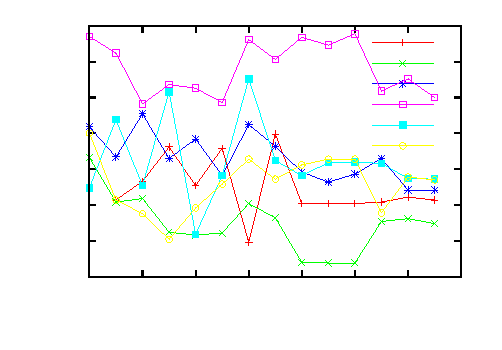
\includegraphics{costsA}}%
    \gplfronttext
  \end{picture}%
\endgroup

  \caption{Timetabling solutions costs vs.\ 
           $\mathsf{conf}$\label{costsA}}
\end{figure}

\begin{figure}
  \centering
  % GNUPLOT: LaTeX picture with Postscript
\begingroup
  \makeatletter
  \providecommand\color[2][]{%
    \GenericError{(gnuplot) \space\space\space\@spaces}{%
      Package color not loaded in conjunction with
      terminal option `colourtext'%
    }{See the gnuplot documentation for explanation.%
    }{Either use 'blacktext' in gnuplot or load the package
      color.sty in LaTeX.}%
    \renewcommand\color[2][]{}%
  }%
  \providecommand\includegraphics[2][]{%
    \GenericError{(gnuplot) \space\space\space\@spaces}{%
      Package graphicx or graphics not loaded%
    }{See the gnuplot documentation for explanation.%
    }{The gnuplot epslatex terminal needs graphicx.sty or graphics.sty.}%
    \renewcommand\includegraphics[2][]{}%
  }%
  \providecommand\rotatebox[2]{#2}%
  \@ifundefined{ifGPcolor}{%
    \newif\ifGPcolor
    \GPcolortrue
  }{}%
  \@ifundefined{ifGPblacktext}{%
    \newif\ifGPblacktext
    \GPblacktexttrue
  }{}%
  % define a \g@addto@macro without @ in the name:
  \let\gplgaddtomacro\g@addto@macro
  % define empty templates for all commands taking text:
  \gdef\gplbacktext{}%
  \gdef\gplfronttext{}%
  \makeatother
  \ifGPblacktext
    % no textcolor at all
    \def\colorrgb#1{}%
    \def\colorgray#1{}%
  \else
    % gray or color?
    \ifGPcolor
      \def\colorrgb#1{\color[rgb]{#1}}%
      \def\colorgray#1{\color[gray]{#1}}%
      \expandafter\def\csname LTw\endcsname{\color{white}}%
      \expandafter\def\csname LTb\endcsname{\color{black}}%
      \expandafter\def\csname LTa\endcsname{\color{black}}%
      \expandafter\def\csname LT0\endcsname{\color[rgb]{1,0,0}}%
      \expandafter\def\csname LT1\endcsname{\color[rgb]{0,1,0}}%
      \expandafter\def\csname LT2\endcsname{\color[rgb]{0,0,1}}%
      \expandafter\def\csname LT3\endcsname{\color[rgb]{1,0,1}}%
      \expandafter\def\csname LT4\endcsname{\color[rgb]{0,1,1}}%
      \expandafter\def\csname LT5\endcsname{\color[rgb]{1,1,0}}%
      \expandafter\def\csname LT6\endcsname{\color[rgb]{0,0,0}}%
      \expandafter\def\csname LT7\endcsname{\color[rgb]{1,0.3,0}}%
      \expandafter\def\csname LT8\endcsname{\color[rgb]{0.5,0.5,0.5}}%
    \else
      % gray
      \def\colorrgb#1{\color{black}}%
      \def\colorgray#1{\color[gray]{#1}}%
      \expandafter\def\csname LTw\endcsname{\color{white}}%
      \expandafter\def\csname LTb\endcsname{\color{black}}%
      \expandafter\def\csname LTa\endcsname{\color{black}}%
      \expandafter\def\csname LT0\endcsname{\color{black}}%
      \expandafter\def\csname LT1\endcsname{\color{black}}%
      \expandafter\def\csname LT2\endcsname{\color{black}}%
      \expandafter\def\csname LT3\endcsname{\color{black}}%
      \expandafter\def\csname LT4\endcsname{\color{black}}%
      \expandafter\def\csname LT5\endcsname{\color{black}}%
      \expandafter\def\csname LT6\endcsname{\color{black}}%
      \expandafter\def\csname LT7\endcsname{\color{black}}%
      \expandafter\def\csname LT8\endcsname{\color{black}}%
    \fi
  \fi
  \setlength{\unitlength}{0.0500bp}%
  \begin{picture}(4824.00,3376.80)%
    \gplgaddtomacro\gplbacktext{%
      \csname LTb\endcsname%
      \put(858,704){\makebox(0,0)[r]{\strut{}$\scriptstyle{0}$}}%
      \put(858,923){\makebox(0,0)[r]{\strut{}$\scriptstyle{200}$}}%
      \put(858,1142){\makebox(0,0)[r]{\strut{}$\scriptstyle{400}$}}%
      \put(858,1361){\makebox(0,0)[r]{\strut{}$\scriptstyle{600}$}}%
      \put(858,1580){\makebox(0,0)[r]{\strut{}$\scriptstyle{800}$}}%
      \put(858,1799){\makebox(0,0)[r]{\strut{}$\scriptstyle{1000}$}}%
      \put(858,2017){\makebox(0,0)[r]{\strut{}$\scriptstyle{1200}$}}%
      \put(858,2236){\makebox(0,0)[r]{\strut{}$\scriptstyle{1400}$}}%
      \put(858,2455){\makebox(0,0)[r]{\strut{}$\scriptstyle{1600}$}}%
      \put(858,2674){\makebox(0,0)[r]{\strut{}$\scriptstyle{1800}$}}%
      \put(858,2893){\makebox(0,0)[r]{\strut{}$\scriptstyle{2000}$}}%
      \put(858,3112){\makebox(0,0)[r]{\strut{}$\scriptstyle{2200}$}}%
      \put(990,484){\makebox(0,0){\strut{}$\scriptstyle{0}$}}%
      \put(1481,484){\makebox(0,0){\strut{}$\scriptstyle{20}$}}%
      \put(1972,484){\makebox(0,0){\strut{}$\scriptstyle{40}$}}%
      \put(2463,484){\makebox(0,0){\strut{}$\scriptstyle{60}$}}%
      \put(2954,484){\makebox(0,0){\strut{}$\scriptstyle{80}$}}%
      \put(3445,484){\makebox(0,0){\strut{}$\scriptstyle{100}$}}%
      \put(3936,484){\makebox(0,0){\strut{}$\scriptstyle{120}$}}%
      \put(4427,484){\makebox(0,0){\strut{}$\scriptstyle{140}$}}%
      \put(286,1908){\rotatebox{-270}{\makebox(0,0){\strut{}Solution Cost}}}%
      \put(2708,154){\makebox(0,0){\strut{}$\mathsf{conf}$}}%
    }%
    \gplgaddtomacro\gplfronttext{%
      \csname LTb\endcsname%
      \put(1925,2939){\makebox(0,0)[r]{\strut{}\textsf{\scriptsize Fis0506-1}}}%
      \csname LTb\endcsname%
      \put(1925,2719){\makebox(0,0)[r]{\strut{}\textsf{\scriptsize Ing0405-3}}}%
      \csname LTb\endcsname%
      \put(1925,2499){\makebox(0,0)[r]{\strut{}\textsf{\scriptsize Let0405-1}}}%
      \csname LTb\endcsname%
      \put(1925,2279){\makebox(0,0)[r]{\strut{}\textsf{\scriptsize Ing0506-1}}}%
      \csname LTb\endcsname%
      \put(3440,2939){\makebox(0,0)[r]{\strut{}\textsf{\scriptsize Ing0607-2}}}%
      \csname LTb\endcsname%
      \put(3440,2719){\makebox(0,0)[r]{\strut{}\textsf{\scriptsize Ing0607-3}}}%
      \csname LTb\endcsname%
      \put(3440,2499){\makebox(0,0)[r]{\strut{}\textsf{\scriptsize Fis0506-2}}}%
      \csname LTb\endcsname%
      \put(3440,2279){\makebox(0,0)[r]{\strut{}\textsf{\scriptsize Let0506-2}}}%
    }%
    \gplbacktext
    \put(0,0){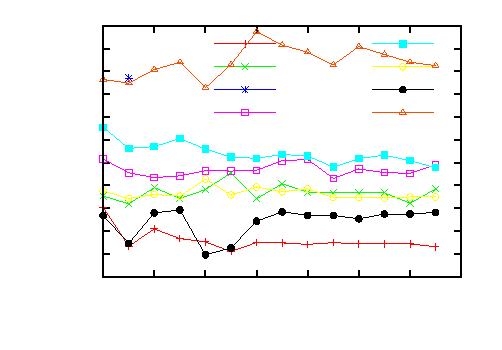
\includegraphics{costsB}}%
    \gplfronttext
  \end{picture}%
\endgroup

  \caption{Solutions for the rest of the ITC
           instances\label{costsB}}
\end{figure}

It was expected that for high $\mathsf{conf}$ values the
results would be more constant, as the search process
approximates the default depth-first-search (DFS). For the
marginal low values, e.g.\ $\mathsf{conf} = 0$, search is
completely stochastic and the results are worse on overage,
as we have higher solution costs. However, the evaluations
for intermediate $\mathsf{conf}$ values, e.g.\ 
$\mathsf{conf} \approx 20$, are more promising. Remember
that an intermediate $\mathsf{conf}$ value favors the
selection which corresponds to the best heuristic
evaluation, \emph{but} it also gives room to other
selections (the ``outsiders'') as their probabilities are
not zero.

The automatic selection of the best $\mathsf{conf}$ is an
open question here; in the last sections, \textsc{PoPS}
finds automatically the best $\mathsf{conf}$ values.

In practice, as shown in Fig.\ \ref{costsA} and
\ref{costsB}, a $\mathsf{conf}$ value around $100$ actually
represents infinity, because search tends to produce the
same solutions for $\mathsf{conf} \geq 100$.

It is worth to mention that in Fig.~\ref{costsB} the only
solution found for the \textsf{Let0405-1} instance, depicted
with an asterisk~\textcolor{blue}{$*$}, was for an
intermediate $\mathsf{conf} = 10$.

\subsection{Radio link frequency assignment}

Another important real problem is the frequency assignment,
in which we have to assign a frequency to each radio
transmitter with the objective to minimize the interference.
The interference is minimized by assigning different
frequencies to every two transmitters that are close to each
other.

The Centre Electronique de l'Armement (CELAR) provides a set
of real datasets for this NP-hard problem.\cite{Cabon1999}
We chose to solve the five so-called ``MAX'' problem
instances, namely \textsf{SCEN06}--\textsf{SCEN10}, in
which, generally speaking, we try to maximize the number of
the satisfied soft constraints. Similarly to the above
course scheduling experiments, as \emph{variables ordering
heuristic} we used minimum remaining values and degree for
tie breaking, and we randomized it using the function in
Lemma~\ref{exponential}.

For each of these instances, we had 15 minutes to explore
the search space. We recorded the best (lowest) solution
costs found so far in Fig.~\ref{CELAR} for several
$\mathsf{conf}$ values. Approximately the same as in course
scheduling, the lowest solution costs occur around
$\mathsf{conf} \approx 10$, which gives better results on
average than the marginal $\mathsf{conf}$ values. This means
that we achieve best results when the confidence to our
heuristic is neither too high nor very low.

\begin{figure}
  \centering
  % GNUPLOT: LaTeX picture with Postscript
\begingroup
  \makeatletter
  \providecommand\color[2][]{%
    \GenericError{(gnuplot) \space\space\space\@spaces}{%
      Package color not loaded in conjunction with
      terminal option `colourtext'%
    }{See the gnuplot documentation for explanation.%
    }{Either use 'blacktext' in gnuplot or load the package
      color.sty in LaTeX.}%
    \renewcommand\color[2][]{}%
  }%
  \providecommand\includegraphics[2][]{%
    \GenericError{(gnuplot) \space\space\space\@spaces}{%
      Package graphicx or graphics not loaded%
    }{See the gnuplot documentation for explanation.%
    }{The gnuplot epslatex terminal needs graphicx.sty or graphics.sty.}%
    \renewcommand\includegraphics[2][]{}%
  }%
  \providecommand\rotatebox[2]{#2}%
  \@ifundefined{ifGPcolor}{%
    \newif\ifGPcolor
    \GPcolortrue
  }{}%
  \@ifundefined{ifGPblacktext}{%
    \newif\ifGPblacktext
    \GPblacktexttrue
  }{}%
  % define a \g@addto@macro without @ in the name:
  \let\gplgaddtomacro\g@addto@macro
  % define empty templates for all commands taking text:
  \gdef\gplbacktext{}%
  \gdef\gplfronttext{}%
  \makeatother
  \ifGPblacktext
    % no textcolor at all
    \def\colorrgb#1{}%
    \def\colorgray#1{}%
  \else
    % gray or color?
    \ifGPcolor
      \def\colorrgb#1{\color[rgb]{#1}}%
      \def\colorgray#1{\color[gray]{#1}}%
      \expandafter\def\csname LTw\endcsname{\color{white}}%
      \expandafter\def\csname LTb\endcsname{\color{black}}%
      \expandafter\def\csname LTa\endcsname{\color{black}}%
      \expandafter\def\csname LT0\endcsname{\color[rgb]{1,0,0}}%
      \expandafter\def\csname LT1\endcsname{\color[rgb]{0,1,0}}%
      \expandafter\def\csname LT2\endcsname{\color[rgb]{0,0,1}}%
      \expandafter\def\csname LT3\endcsname{\color[rgb]{1,0,1}}%
      \expandafter\def\csname LT4\endcsname{\color[rgb]{0,1,1}}%
      \expandafter\def\csname LT5\endcsname{\color[rgb]{1,1,0}}%
      \expandafter\def\csname LT6\endcsname{\color[rgb]{0,0,0}}%
      \expandafter\def\csname LT7\endcsname{\color[rgb]{1,0.3,0}}%
      \expandafter\def\csname LT8\endcsname{\color[rgb]{0.5,0.5,0.5}}%
    \else
      % gray
      \def\colorrgb#1{\color{black}}%
      \def\colorgray#1{\color[gray]{#1}}%
      \expandafter\def\csname LTw\endcsname{\color{white}}%
      \expandafter\def\csname LTb\endcsname{\color{black}}%
      \expandafter\def\csname LTa\endcsname{\color{black}}%
      \expandafter\def\csname LT0\endcsname{\color{black}}%
      \expandafter\def\csname LT1\endcsname{\color{black}}%
      \expandafter\def\csname LT2\endcsname{\color{black}}%
      \expandafter\def\csname LT3\endcsname{\color{black}}%
      \expandafter\def\csname LT4\endcsname{\color{black}}%
      \expandafter\def\csname LT5\endcsname{\color{black}}%
      \expandafter\def\csname LT6\endcsname{\color{black}}%
      \expandafter\def\csname LT7\endcsname{\color{black}}%
      \expandafter\def\csname LT8\endcsname{\color{black}}%
    \fi
  \fi
  \setlength{\unitlength}{0.0500bp}%
  \begin{picture}(4750.00,4750.00)%
    \gplgaddtomacro\gplbacktext{%
      \csname LTb\endcsname%
      \put(660,3910){\makebox(0,0)[r]{\strut{}$\scriptstyle{280000}$}}%
      \put(660,4150){\makebox(0,0)[r]{\strut{}$\scriptstyle{300000}$}}%
      \put(660,4389){\makebox(0,0)[r]{\strut{}$\scriptstyle{320000}$}}%
      \put(660,4629){\makebox(0,0)[r]{\strut{}$\scriptstyle{340000}$}}%
      \put(792,3690){\makebox(0,0){\strut{}}}%
      \put(1380,3690){\makebox(0,0){\strut{}}}%
      \put(1969,3690){\makebox(0,0){\strut{}}}%
      \put(2557,3690){\makebox(0,0){\strut{}}}%
      \put(3146,3690){\makebox(0,0){\strut{}}}%
      \put(3734,3690){\makebox(0,0){\strut{}}}%
      \put(4323,3690){\makebox(0,0){\strut{}}}%
      \put(3967,4204){\makebox(0,0)[l]{\strut{}\textsf{\scriptsize SCEN07}}}%
    }%
    \gplgaddtomacro\gplfronttext{%
    }%
    \gplgaddtomacro\gplbacktext{%
      \csname LTb\endcsname%
      \put(660,3100){\makebox(0,0)[r]{\strut{}$\scriptstyle{10000}$}}%
      \put(660,3380){\makebox(0,0)[r]{\strut{}$\scriptstyle{11000}$}}%
      \put(660,3659){\makebox(0,0)[r]{\strut{}$\scriptstyle{12000}$}}%
      \put(792,2740){\makebox(0,0){\strut{}}}%
      \put(1380,2740){\makebox(0,0){\strut{}}}%
      \put(1969,2740){\makebox(0,0){\strut{}}}%
      \put(2557,2740){\makebox(0,0){\strut{}}}%
      \put(3146,2740){\makebox(0,0){\strut{}}}%
      \put(3734,2740){\makebox(0,0){\strut{}}}%
      \put(4323,2740){\makebox(0,0){\strut{}}}%
      \put(3967,3212){\makebox(0,0)[l]{\strut{}\textsf{\scriptsize SCEN10}}}%
    }%
    \gplgaddtomacro\gplfronttext{%
    }%
    \gplgaddtomacro\gplbacktext{%
      \csname LTb\endcsname%
      \put(660,2010){\makebox(0,0)[r]{\strut{}$\scriptstyle{460}$}}%
      \put(660,2220){\makebox(0,0)[r]{\strut{}$\scriptstyle{480}$}}%
      \put(660,2430){\makebox(0,0)[r]{\strut{}$\scriptstyle{500}$}}%
      \put(660,2639){\makebox(0,0)[r]{\strut{}$\scriptstyle{520}$}}%
      \put(660,2849){\makebox(0,0)[r]{\strut{}$\scriptstyle{540}$}}%
      \put(792,1790){\makebox(0,0){\strut{}}}%
      \put(1380,1790){\makebox(0,0){\strut{}}}%
      \put(1969,1790){\makebox(0,0){\strut{}}}%
      \put(2557,1790){\makebox(0,0){\strut{}}}%
      \put(3146,1790){\makebox(0,0){\strut{}}}%
      \put(3734,1790){\makebox(0,0){\strut{}}}%
      \put(4323,1790){\makebox(0,0){\strut{}}}%
      \put(154,2429){\rotatebox{-270}{\makebox(0,0){\strut{}Solution Cost (thousands)}}}%
      \put(3967,2346){\makebox(0,0)[l]{\strut{}\textsf{\scriptsize SCEN09}}}%
    }%
    \gplgaddtomacro\gplfronttext{%
    }%
    \gplgaddtomacro\gplbacktext{%
      \csname LTb\endcsname%
      \put(660,1200){\makebox(0,0)[r]{\strut{}$\scriptstyle{170}$}}%
      \put(660,1480){\makebox(0,0)[r]{\strut{}$\scriptstyle{180}$}}%
      \put(660,1760){\makebox(0,0)[r]{\strut{}$\scriptstyle{190}$}}%
      \put(792,840){\makebox(0,0){\strut{}}}%
      \put(1380,840){\makebox(0,0){\strut{}}}%
      \put(1969,840){\makebox(0,0){\strut{}}}%
      \put(2557,840){\makebox(0,0){\strut{}}}%
      \put(3146,840){\makebox(0,0){\strut{}}}%
      \put(3734,840){\makebox(0,0){\strut{}}}%
      \put(4323,840){\makebox(0,0){\strut{}}}%
      \put(3967,1354){\makebox(0,0)[l]{\strut{}\textsf{\scriptsize SCEN06}}}%
    }%
    \gplgaddtomacro\gplfronttext{%
    }%
    \gplgaddtomacro\gplbacktext{%
      \csname LTb\endcsname%
      \put(660,568){\makebox(0,0)[r]{\strut{}$\scriptstyle{8.4}$}}%
      \put(660,823){\makebox(0,0)[r]{\strut{}$\scriptstyle{8.6}$}}%
      \put(792,220){\makebox(0,0){\strut{}$\scriptstyle{0}$}}%
      \put(1380,220){\makebox(0,0){\strut{}$\scriptstyle{20}$}}%
      \put(1969,220){\makebox(0,0){\strut{}$\scriptstyle{40}$}}%
      \put(2557,220){\makebox(0,0){\strut{}$\scriptstyle{60}$}}%
      \put(3146,220){\makebox(0,0){\strut{}$\scriptstyle{80}$}}%
      \put(3734,220){\makebox(0,0){\strut{}$\scriptstyle{100}$}}%
      \put(4323,220){\makebox(0,0){\strut{}$\scriptstyle{120}$}}%
      \put(2704,-110){\makebox(0,0){\strut{}$\mathsf{conf}$}}%
      \put(3967,823){\makebox(0,0)[l]{\strut{}\textsf{\scriptsize SCEN08}}}%
    }%
    \gplgaddtomacro\gplfronttext{%
    }%
    \gplbacktext
    \put(0,0){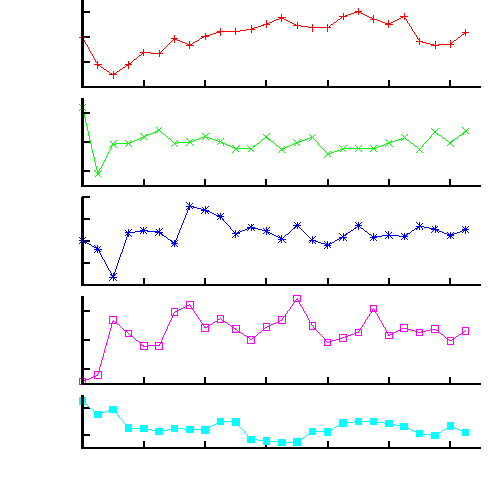
\includegraphics{CELAR}}%
    \gplfronttext
  \end{picture}%
\endgroup

  \caption{Unsatisfied soft constraints increase
           cost\label{CELAR}}
\end{figure}

\subsection{\PopsSample{} during hard optimization}

The $\mathsf{conf}$ parameter can refine any search method
that adopts our heuristic framework. The \textsc{PopsSample}
method goes a step further: it incorporates our heuristic
\emph{confidence semantics} into its search engine.

In order to solve the first university course timetabling
instance (\textsf{Fis0506-1} of Section~\ref{ITC}), we
invoked \textsc{PopsSample} for various
$\mathsf{PieceToCover}$ and $\mathsf{conf}$ values and we
plotted the best solution costs found in Figure~\ref{ITC1}.
The third dimension is the \emph{cost} of the solutions
found: the lower the solution cost is, the more qualitative
timetable is produced.

\begin{figure}
  \centering
  % GNUPLOT: LaTeX picture with Postscript
\begingroup
  \makeatletter
  \providecommand\color[2][]{%
    \GenericError{(gnuplot) \space\space\space\@spaces}{%
      Package color not loaded in conjunction with
      terminal option `colourtext'%
    }{See the gnuplot documentation for explanation.%
    }{Either use 'blacktext' in gnuplot or load the package
      color.sty in LaTeX.}%
    \renewcommand\color[2][]{}%
  }%
  \providecommand\includegraphics[2][]{%
    \GenericError{(gnuplot) \space\space\space\@spaces}{%
      Package graphicx or graphics not loaded%
    }{See the gnuplot documentation for explanation.%
    }{The gnuplot epslatex terminal needs graphicx.sty or graphics.sty.}%
    \renewcommand\includegraphics[2][]{}%
  }%
  \providecommand\rotatebox[2]{#2}%
  \@ifundefined{ifGPcolor}{%
    \newif\ifGPcolor
    \GPcolortrue
  }{}%
  \@ifundefined{ifGPblacktext}{%
    \newif\ifGPblacktext
    \GPblacktexttrue
  }{}%
  % define a \g@addto@macro without @ in the name:
  \let\gplgaddtomacro\g@addto@macro
  % define empty templates for all commands taking text:
  \gdef\gplbacktext{}%
  \gdef\gplfronttext{}%
  \makeatother
  \ifGPblacktext
    % no textcolor at all
    \def\colorrgb#1{}%
    \def\colorgray#1{}%
  \else
    % gray or color?
    \ifGPcolor
      \def\colorrgb#1{\color[rgb]{#1}}%
      \def\colorgray#1{\color[gray]{#1}}%
      \expandafter\def\csname LTw\endcsname{\color{white}}%
      \expandafter\def\csname LTb\endcsname{\color{black}}%
      \expandafter\def\csname LTa\endcsname{\color{black}}%
      \expandafter\def\csname LT0\endcsname{\color[rgb]{1,0,0}}%
      \expandafter\def\csname LT1\endcsname{\color[rgb]{0,1,0}}%
      \expandafter\def\csname LT2\endcsname{\color[rgb]{0,0,1}}%
      \expandafter\def\csname LT3\endcsname{\color[rgb]{1,0,1}}%
      \expandafter\def\csname LT4\endcsname{\color[rgb]{0,1,1}}%
      \expandafter\def\csname LT5\endcsname{\color[rgb]{1,1,0}}%
      \expandafter\def\csname LT6\endcsname{\color[rgb]{0,0,0}}%
      \expandafter\def\csname LT7\endcsname{\color[rgb]{1,0.3,0}}%
      \expandafter\def\csname LT8\endcsname{\color[rgb]{0.5,0.5,0.5}}%
    \else
      % gray
      \def\colorrgb#1{\color{black}}%
      \def\colorgray#1{\color[gray]{#1}}%
      \expandafter\def\csname LTw\endcsname{\color{white}}%
      \expandafter\def\csname LTb\endcsname{\color{black}}%
      \expandafter\def\csname LTa\endcsname{\color{black}}%
      \expandafter\def\csname LT0\endcsname{\color{black}}%
      \expandafter\def\csname LT1\endcsname{\color{black}}%
      \expandafter\def\csname LT2\endcsname{\color{black}}%
      \expandafter\def\csname LT3\endcsname{\color{black}}%
      \expandafter\def\csname LT4\endcsname{\color{black}}%
      \expandafter\def\csname LT5\endcsname{\color{black}}%
      \expandafter\def\csname LT6\endcsname{\color{black}}%
      \expandafter\def\csname LT7\endcsname{\color{black}}%
      \expandafter\def\csname LT8\endcsname{\color{black}}%
    \fi
  \fi
  \setlength{\unitlength}{0.0500bp}%
  \begin{picture}(4824.00,3376.80)%
    \gplgaddtomacro\gplbacktext{%
      \csname LTb\endcsname%
      \put(3970,2058){\makebox(0,0)[l]{\strut{}\textcolor{green}{DFS}}}%
      \put(3970,1851){\makebox(0,0)[l]{\strut{}\textcolor{cyan}{Iterative}}}%
      \put(3970,1677){\makebox(0,0)[l]{\strut{}\textcolor{cyan}{Broadening}}}%
      \put(3970,1414){\makebox(0,0)[l]{\strut{}\textcolor{orange}{LDS}}}%
      \put(450,913){\rotatebox{-15}{\makebox(0,0)[l]{\strut{}$\mathsf{PieceToCover}$}}}%
    }%
    \gplgaddtomacro\gplfronttext{%
      \csname LTb\endcsname%
      \put(1612,838){\makebox(0,0)[r]{\strut{}$\scriptstyle{0}$}}%
      \put(1205,954){\makebox(0,0)[r]{\strut{}$\scriptstyle{0.5}$}}%
      \put(798,1071){\makebox(0,0)[r]{\strut{}$\scriptstyle{1}$}}%
      \put(3983,958){\makebox(0,0){\strut{}$\scriptstyle{0}$}}%
      \put(3663,946){\makebox(0,0){\strut{}$\scriptstyle{20}$}}%
      \put(3344,934){\makebox(0,0){\strut{}$\scriptstyle{40}$}}%
      \put(3024,922){\makebox(0,0){\strut{}$\scriptstyle{60}$}}%
      \put(2704,910){\makebox(0,0){\strut{}$\scriptstyle{80}$}}%
      \put(2385,898){\makebox(0,0){\strut{}$\scriptstyle{100}$}}%
      \put(2066,886){\makebox(0,0){\strut{}$\scriptstyle{120}$}}%
      \put(1746,874){\makebox(0,0){\strut{}$\scriptstyle{140}$}}%
      \put(2866,659){\makebox(0,0){\strut{}$\mathsf{conf}$}}%
      \put(760,1171){\makebox(0,0)[r]{\strut{}$\scriptstyle{50}$}}%
      \put(760,1346){\makebox(0,0)[r]{\strut{}$\scriptstyle{100}$}}%
      \put(760,1522){\makebox(0,0)[r]{\strut{}$\scriptstyle{150}$}}%
      \put(760,1697){\makebox(0,0)[r]{\strut{}$\scriptstyle{200}$}}%
      \put(760,1871){\makebox(0,0)[r]{\strut{}$\scriptstyle{250}$}}%
      \put(760,2047){\makebox(0,0)[r]{\strut{}$\scriptstyle{300}$}}%
      \put(760,2222){\makebox(0,0)[r]{\strut{}$\scriptstyle{350}$}}%
      \put(760,2398){\makebox(0,0)[r]{\strut{}$\scriptstyle{400}$}}%
      \put(760,2573){\makebox(0,0)[r]{\strut{}$\scriptstyle{450}$}}%
      \put(358,1871){\rotatebox{-270}{\makebox(0,0){\strut{}Solution Cost}}}%
    }%
    \gplbacktext
    \put(0,0){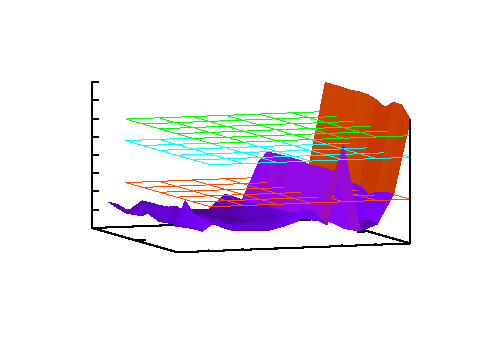
\includegraphics{ITC1}}%
    \gplfronttext
  \end{picture}%
\endgroup

  \caption{{\normalfont\textsc{PopsSample}} for the first
           ITC instance\label{ITC1}}
\end{figure}

In the same graphs we include some of the well-known search
methods results, such as DFS, LDS, and Iterative Broadening,
implemented in the same solver, with only their best
solution cost depicted as a plane grid, in order to make
comparisons easily.

\subsection{\PoPS{} vs.\ other search methods}

In the above sections, it was not easy to figure out which
is the best $\mathsf{PieceToCover}$ and $\mathsf{conf}$
combination. That is why we employed \textsc{PoPS} to solve
the fourteen course timetabling instances.

As described in Section~\ref{sampling}, \textsc{PoPS} uses
several $\mathsf{conf}$ values and favours the most fruitful
ones. We used five $\mathsf{conf}$ samples, i.e.\ $0$, $25$,
$50$, $75$, and $100$, by setting $\mathsf{SamplesNum}$
equal to $5$. In this way, \textsc{PoPS} constructed
solutions with lower costs than the other methods, except
for the fifth instance, as illustrated in
Table~\ref{PopsItc}.

In this section, we used least constraining value as
\textsc{ValuesOrderHeuristic}, and we randomized it using
the function in Lemma~\ref{exponential}. The time limit for
all the methods was set to 15 minutes.

\begin{table}
  \tbl{Solution costs for fourteen ITC
       instances\label{PopsItc}}
  {\begin{tabular}{ccccc}
    \toprule
              Instance & \textsc{PoPS} & LDS & DFS & It.\ Broad. \\
    \colrule
    \textsf{Fis0506-1} & $\mathit{105}$ & $171$ &  $345$ & $286$ \\
    \textsf{Ing0203-2} & $\mathit{241}$ & $288$ &  $698$ & $321$ \\
    \textsf{Ing0304-1} & $\mathit{279}$ & $307$ &  $578$ & $353$ \\
    \textsf{Ing0405-3} & $\mathit{195}$ & $215$ &  $817$ & $235$ \\
    \textsf{Let0405-1} & $655$ & $\mathit{627}$ &    X   &   X   \\
    \textsf{Ing0506-1} & $\mathit{307}$ & $311$ &  $812$ & $342$ \\
    \textsf{Ing0607-2} & $\mathit{282}$ & $283$ & $1184$ & $328$ \\
    \textsf{Ing0607-3} & $\mathit{223}$ & $239$ &  $635$ & $262$ \\
    \textsf{Ing0304-3} & $\mathit{288}$ & $294$ &  $675$ & $370$ \\
    \textsf{Ing0405-2} & $\mathit{265}$ & $284$ &  $877$ & $344$ \\
    \textsf{Fis0506-2} &  $\mathit{12}$ &  $33$ &  $486$ &  $34$ \\
    \textsf{Let0506-2} & $\mathit{713}$ & $783$ & $1621$ & $937$ \\
    \textsf{Ing0506-3} & $\mathit{231}$ & $256$ &  $660$ & $280$ \\
    \textsf{Ing0708-1} & $\mathit{223}$ & $227$ &  $660$ & $264$ \\
    \botrule
  \end{tabular}}
\end{table}


\section{Conclusions and Perspectives}

The initial contribution of this work is the provision of an
interface that everyone can use to define their search
methods. Except from easing the declaration of custom search
methods, we elaborated on the algorithm behind the scenes
supporting our interface in an open source solver.

We also presented a well-founded paradigm to exploit both
stochastic and deterministic heuristics. Empirical
evaluations showed that our hybrid approach can produce
better results than fully random or fully deterministic
methodologies.

In order to achieve this, we approached and used heuristics
as a \emph{confidence} and \emph{reliability} measure. By
exploiting these heuristic semantics, we were able to
produce a new efficient search method, namely \textsc{PoPS},
that can outperform other methodologies. In general, our
proposed framework gives the opportunity to exploit ``on the
fly'' whichever heuristic confidence fluctuations occur.

In future, it will be challenging to parallelize it, as it
supports a whole grid of strategies, by concurrently
invoking \textsc{PopsSample} with several
$\mathsf{PieceToCover}$ and $\mathsf{conf}$ arguments.

Constraint Programming consists of the CSP \emph{definition}
and \emph{search} phases. A crucial goal in this area is to
make these two phases as independent as possible from each
other.\cite{Freuder2014} The presented search methods
interface was one step into making the search phase more
transparent. But the search phase doesn't include only the
search method; it includes also mechanisms that check if the
constraints are violated and enforces a kind of consistency
between the domains of the variables that are connected via
constraints.\cite{Chen2013}

Therefore, in the next years, it would be also important to
modularize the consistency enforcement part of the search
phase, as we did in this work for the search methods.


\section*{Acknowledgments}

We want to thank Foivos Theocharis who initially built the
search methods library \textsc{Amorgos}, which is available
together with \textsc{Naxos}.\cite{Naxos} We also thank the
anonymous reviewers for their constructive comments.

\bibliographystyle{ws-ijait}
\bibliography{bibliography}


\appendix

\section{An Algorithm that Satisfies Search Methods'
         Goals\label{framework-algorithm}}

In Section~\ref{search-framework} we described a high level
language to define search methods. This framework consists
of goals that support recursion (goals that return another
goal or success) and meta-goals used to combine other goals
in a conjunctive (\textsf{AND}) or disjunctive (\textsf{OR})
manner.

This is a not only a theoretical model; it has been
implemented in a C++ Constraint Programming \textsc{Naxos
Solver}. DFS and Iterative Broadening have been already
declared in \textsc{Naxos} without loosing much of the above
expressiveness, along with many other search methods in the
solver's repository.\cite{Naxos}

The search methods' goals cannot solve by themselves any
CSP; we need a procedure to \emph{satisfy} these goals.
\textsc{Solve} algorithm in Figure~\ref{solve} uses an
advanced ``stack of stacks'' data structure to store goals.
Initially, the stack of stacks contains just a single goal,
e.g.\ \texttt{Broadening}($1$) or
\texttt{Label}($\mathscr{X}$) for DFS, as in
Figure~\ref{a2h}(a).

\begin{figure}
  \centering
  \begin{algorithmic}
    \Function{Solve}{}
      \State \textbf{local variables:}
      \State \quad stacks: the ``stack of stacks'' instance
      \State \quad $\mathit{Goal}$: current goal that has to
                   be satisfied
      \State \quad $\mathit{NextGoal}$: generated goal by
                   current goal's execution
      \State
      \While {time limit has not been reached}
        \If {stacks.top is not empty}
          \State $\mathit{Goal} \gets
                  \mathrm{stacks.top.pop()}$
        \Else
          \State $\mathit{Goal} \gets
                  \mathrm{stacks.top.pending}$
          \State $\mathrm{stacks.top.pending} \gets$
                 get the next goal of the frame that
                 ``pending'' \\ \hspace*{14em} points to
                 \textbf{or} (if there is not such a goal)
                 get \\ \hspace*{14em} the next ``pending''
                 goal of that frame
        \EndIf
        \If {$\mathit{Goal}$ is an AND-goal}
          \State stacks.top.push(2\textsuperscript{nd}
                 subgoal of $\mathit{Goal}$)
          \State stacks.top.push(1\textsuperscript{st}
                 subgoal of $\mathit{Goal}$)
        \ElsIf {$\mathit{Goal}$ is an OR-goal}
          \State stacks.top.push(2\textsuperscript{nd}
                 subgoal of $\mathit{Goal}$)
          \State stacks.push() \Comment Push an empty frame
          \State stacks.top.push(1\textsuperscript{st}
                 subgoal of $\mathit{Goal}$)
          \State $\mathrm{stacks.top.pending} \gets$
                 the goal after the 2\textsuperscript{nd}
                 subgoal in the below frame
        \Else
          \State $\mathit{NextGoal} \gets
                  \mathit{Goal}$.execute()
          \If {$\Call{PropagateConstraints}{}() =
                \mathrm{false}$}
            \State stacks.pop()
            \Comment Backtrack to previous frame
            \If {stacks empty}
              \State \Return failure
            \EndIf
          \ElsIf {$\mathit{NextGoal} \neq \textrm{null}$}
            \State stacks.top.push($\mathit{NextGoal}$)
          \ElsIf {stacks.top is empty \textbf{and}
                  $\mathrm{stacks.top.pending} =
                   \textrm{null}$}
            \State \Return success
          \EndIf
        \EndIf
      \EndWhile
      \State \Return failure
    \EndFunction
  \end{algorithmic}
  \caption{Goals' Satisfaction Algorithm\label{solve}}
\end{figure}

\begin{figure}
  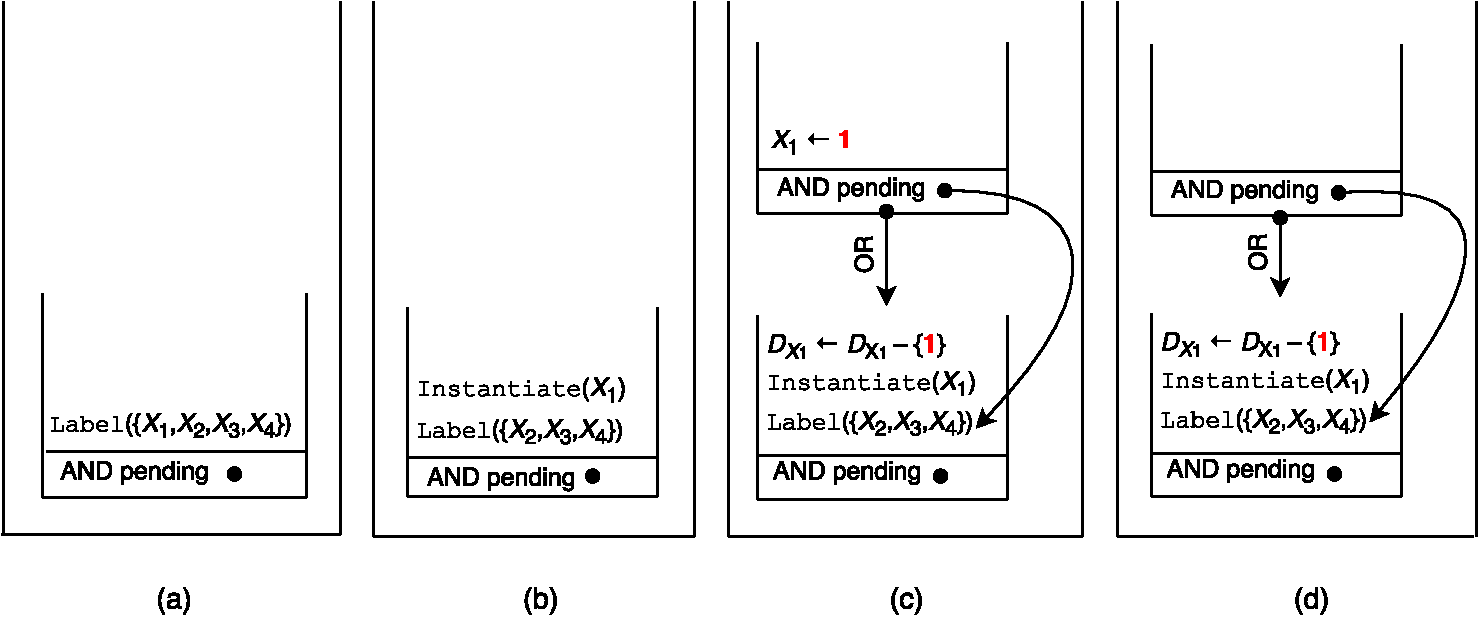
\includegraphics[width=\textwidth]{figures/stacks/abcd}
  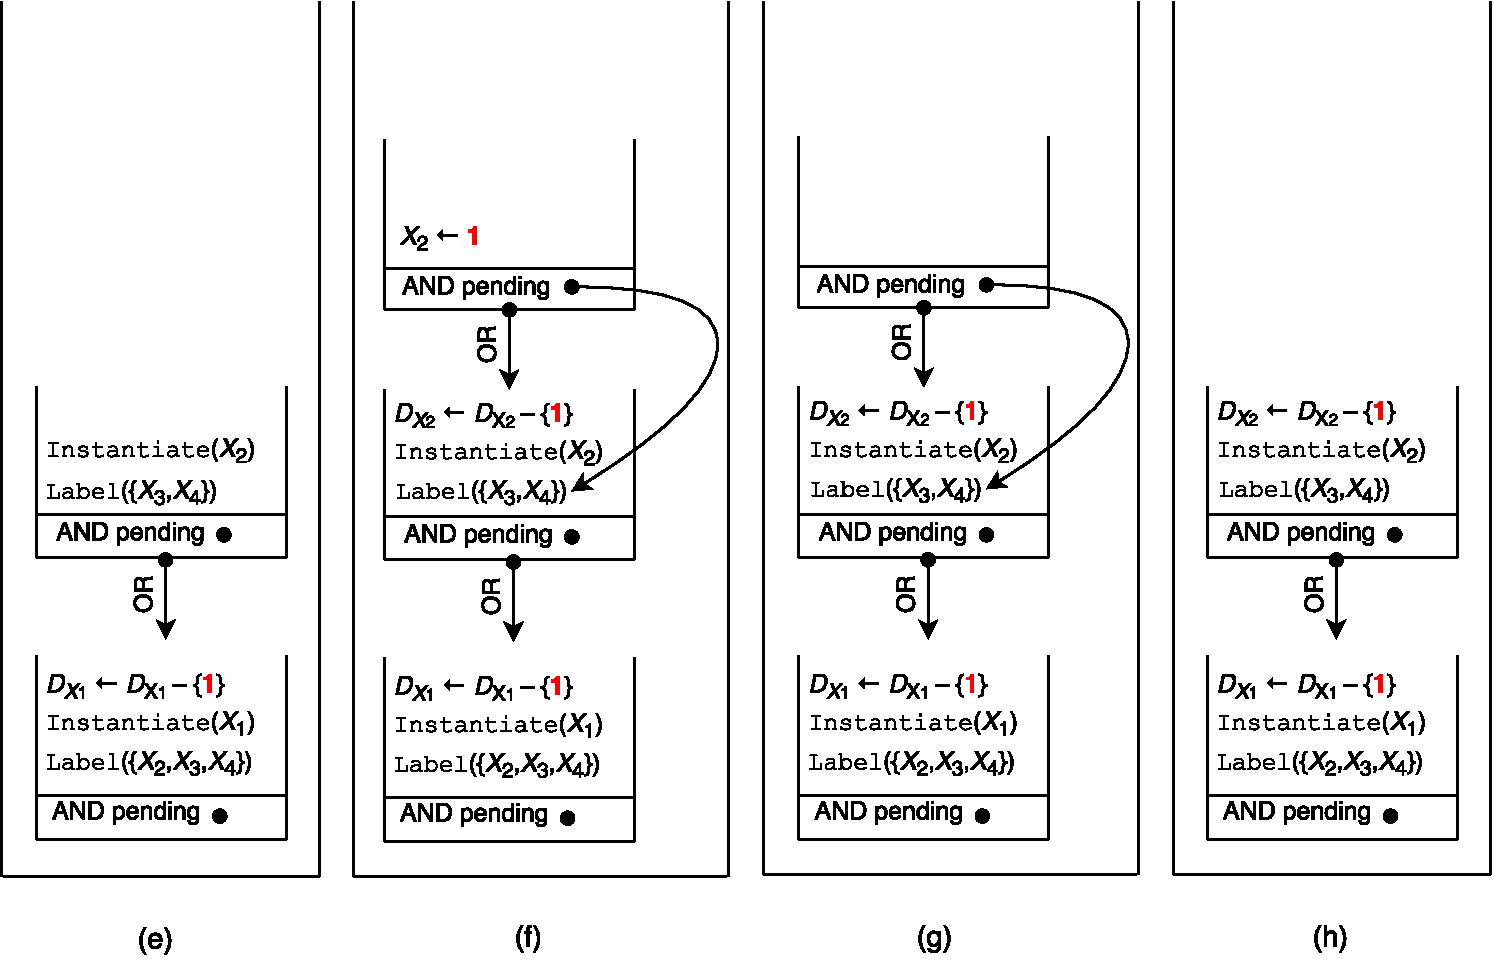
\includegraphics[width=\textwidth]{figures/stacks/efgh}
  \caption{\textsc{Solve} with DFS example: $X_1$
           instantiation and $X_2$ instantiation
           attempt\label{a2h}}
\end{figure}

\subsection{The ``stack of stacks'' data structure}

In order to understand the \textsc{Solve} pseudocode, we
should look closer at the underlying data structure in
Fig.~\ref{a2h}. Each subfigure from (a) to (v) displays a
snapshot of the ``stack of stacks'' main data structure
while trying to satisfy the \texttt{Label}($\mathscr{X}$)
goal for the Thessaly-coloring problem. Here we focus on the
data structure itself.
\begin{itemize}
  \item The ``stack of the stacks'' is outlined by the outer
        borders of each subfigure.
        \begin{itemize}
          \item The frames of the (outer) stack are
                connected with an \textsf{OR} relationship.
        \end{itemize}
  \item Each frame of the outer stack is a stack too,
        containing goals.
        \begin{itemize}
          \item The goals of each (inner) stack are
                connected with an \textsf{AND} relationship.
        \end{itemize}
  \item Each inner stack contains additionally a
        \textsf{pending} pointer.
        \begin{itemize}
          \item It points to the first unsatisfied goal of
                the previous inner stacks.
        \end{itemize}
\end{itemize}

\newcommand{\Solve}{{\normalsize S\footnotesize OLVE}}

\subsection{\Solve{} in a nutshell}

We can see the ``stack of stacks'' data structure inside the
\textsc{Solve} algorithm.
\begin{itemize}
  \item The outer stack corresponds to the ``stacks''
        variable.
  \item The ``stacks.top'' expression corresponds to the top
        frame of the ``stacks.''
  \item The ``stacks.top.pending'' corresponds to the
        pointer of the top frame.
\end{itemize}

The algorithm is wrapped into a \textbf{while} loop. Each
iteration examines another goal.

Inside the loop we have two ``if'' statements. In the first
``if,'' we select the goal that we will attempt to satisfy.
In the second ``if,'' we check if the $\mathit{Goal}$ is a
meta-goal and we handle properly its two subgoals. If it is
not a meta-goal, we simply ``execute()'' it and store the
returned value into the $\mathit{NextGoal}$ variable. A
``null'' returned value means that the executed
$\mathit{Goal}$ did not generate another goal to be
satisfied.

After each $\mathit{Goal}$ execution,
\textsc{PropagateConstraints} is called. A simple
implementation for this function would just check if every
constraint is still valid. If even a single constraint is
violated, \textsc{PropagateConstraints} should return false.
However, as its name implies, \textsc{PropagateConstraints}
can do more just than checking constraints: it may remove
no-good values from the variables and enforce a kind of
``consistency'' between them, but this is beyond the scope
of this paper to further analyze.\cite{Chen2013}

\subsection{\Solve{} in action}

Let's execute \textsc{Solve} to find a solution to the
Thessaly-coloring (Problem~\ref{thessaly-coloring}) using
the DFS method goals (Section~\ref{DFS-goals}). The
snapshots of the ``stack of stacks'' data structure are
visible in the corresponding subfigures of Figures \ref{a2h}
to \ref{tuv}:
\begin{enumerate}
  \item[(a)] Before \textsc{Solve} begins, the first goal to
             be satisfied should be already in the single
             inner stack. In the case of DFS, the initial
             goal is \texttt{Label}($\mathscr{X}$) which in
             Thessaly-coloring is equivalent to
             \texttt{Label}($\{X_1, X_2, X_3, X_4\}$).
  \item[(b)] \textsc{Solve} begins and pops the
             \texttt{Label} goal out of the inner stack and
             executes it. By definition, \texttt{Label}
             returns an \textsf{AND} goal. In other words,
             \texttt{Label} is substituted by an
             \textsf{AND} goal at the inner stack.

             This \textsf{AND} goal is then popped out in
             turn by the next \textsc{Solve} iteration, and
             after its execution it returns its two subgoals
             \texttt{Instantiate}($\{X_1\}$) and
             \texttt{Label}($\{X_2, X_3, X_4\}$). At this
             time, the ``stack of stacks'' looks like
             Fig.~\ref{a2h}(b).
  \item[(c)] By definition, \texttt{Instantiate}($\{X_1\}$)
             is substituted by an \textsf{OR} goal. The
             complete expression for this goal is
             \textsf{OR}($X_1 \! \gets \!
             \textcolor{red}{1}$, \textsf{AND}($D_{X_1} \!\!
             \gets \!\! D_{X_1} \! - \!
             \{\textcolor{red}{1}\}$,\,\texttt{Instantiate}($X_1$))).
             In this case, \textsc{Solve} algorithm should
             cover three requirements.
             \begin{enumerate}
               \item[1.] Execute the first subgoal and all
                         the returned\slash generated goals.
               \item[2.] Execute the ``pending'' goals that
                         were unsatisfied before the
                         \textsf{OR}-goal.
               \item[3.] If the above fail, undo all the
                         actions and execute the second
                         subgoal.
             \end{enumerate}
             In Fig.~\ref{a2h}(c), all three requirements
             have been implemented.
             \begin{enumerate}
               \item[1.] The first subgoal is in the top
                         stack and will be executed in the
                         next iteration.
               \item[2.] The ``pending'' pointer of the top
                         stack points to the next
                         unsatisfied goal.
               \item[3.] Most importantly, a new stack has
                         been created on top of the previous
                         inner stack. The new stack was
                         added in order to isolate the
                         previous inner stack. This would be
                         useful if any of the top stack
                         goals fails: The top stack will be
                         popped, and the second
                         \textsf{OR}-subgoal that is stored
                         in the previous inner stack will be
                         executed.
             \end{enumerate}
             For simplicity reasons, instead of adding the
             whole second subgoal \textsf{AND}($D_{X_1} \!\!
             \gets \!\! D_{X_1} \! - \!
             \{\textcolor{red}{1}\}$,
             \texttt{Instantiate}($X_1$)) into the bottom
             stack in Fig.~\ref{a2h}(c), we ``unwrapped'' it
             and added directly its two subgoals.
  \item[(d)] $X_1 \! \gets \! \textcolor{red}{1}$ is
             executed. This assignment does not violate any
             constraint. This goal did not return another
             goal, so the top stack is now empty.
  \item[(e)] As the top stack is empty, \textsc{Solve} uses
             its ``pending'' pointer to fetch the next goal.
             Therefore, \texttt{Label}($\{X_2, X_3, X_4\}$)
             is fetched and the ``pending'' pointer is moved
             one step further, to the next goal. As there
             aren't any more goals, the top stack
             ``pending'' pointer is assigned the bottom
             stack ``pending'' value, which is ``null.''

             The \texttt{Label} goal is executed and returns
             \textsf{AND}(\texttt{Instantiate}($X_2$),
             \texttt{Label}($\{X_3, X_4\}$)), which is
             executed in turn in the next iteration. The
             result is depicted in Fig.~\ref{a2h}(e).

\begin{figure}
  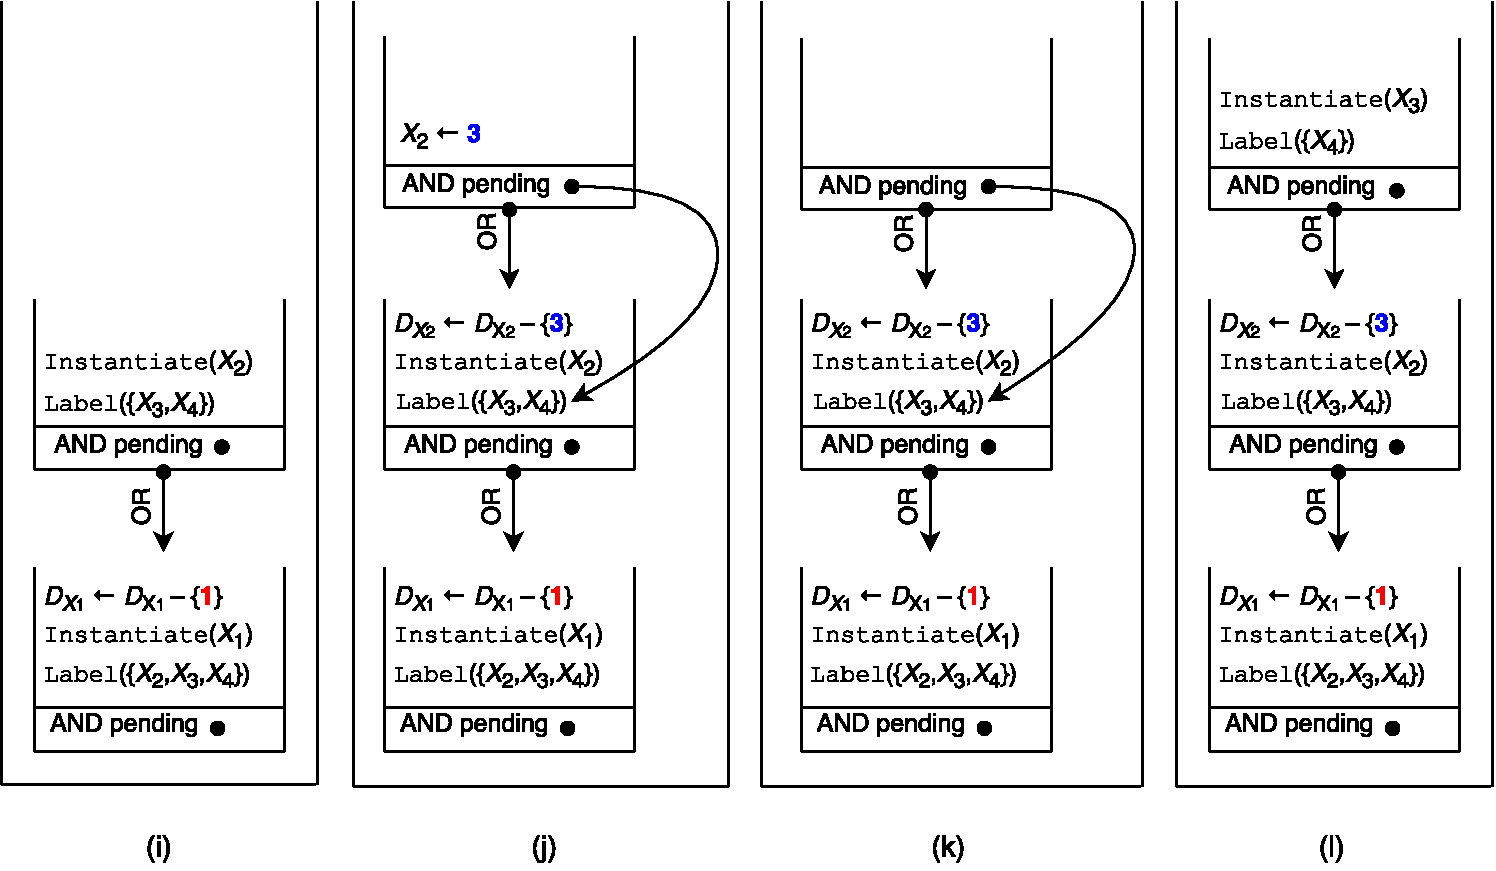
\includegraphics[width=\textwidth]{figures/stacks/ijkl}
  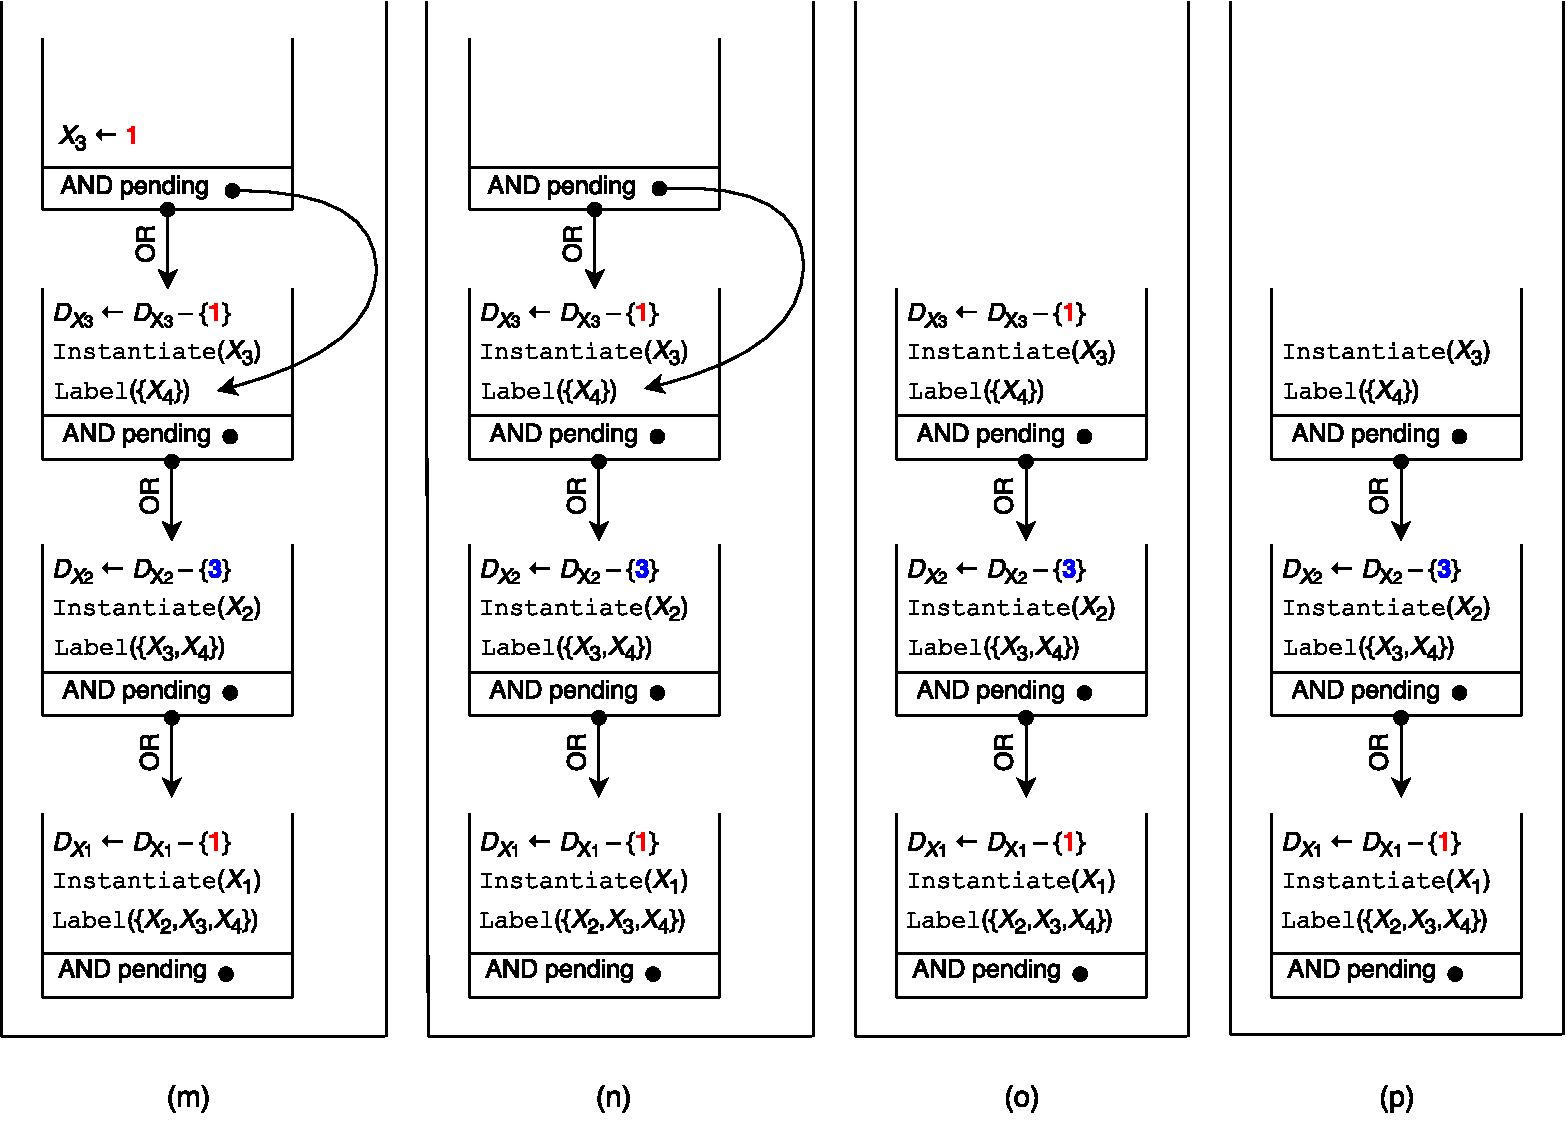
\includegraphics[width=\textwidth]{figures/stacks/mnop}
  \caption{\textsc{Solve} with DFS example: $X_2$ successful
           instantiation and $X_3$ instantiation
           attempt\label{i2p}}
\end{figure}

\begin{figure}
  \centering
  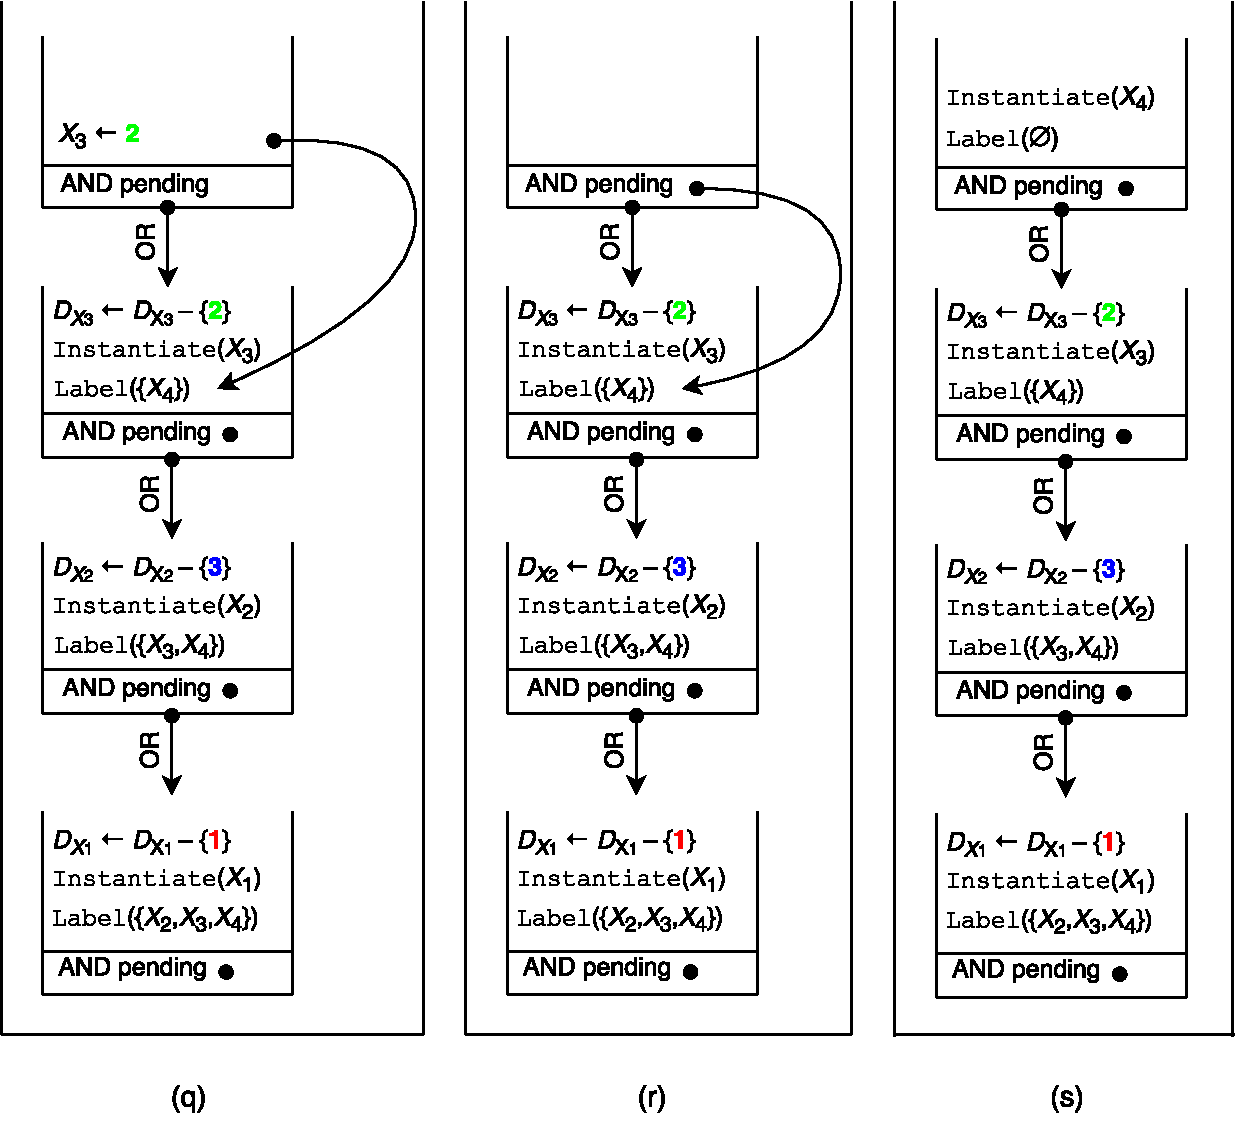
\includegraphics[width=0.9\textwidth]{figures/stacks/qrs}
  \caption{\textsc{Solve} with DFS example: $X_3$ successful
           instantiation\label{qrs}}
\end{figure}

\begin{figure}
  \centering
  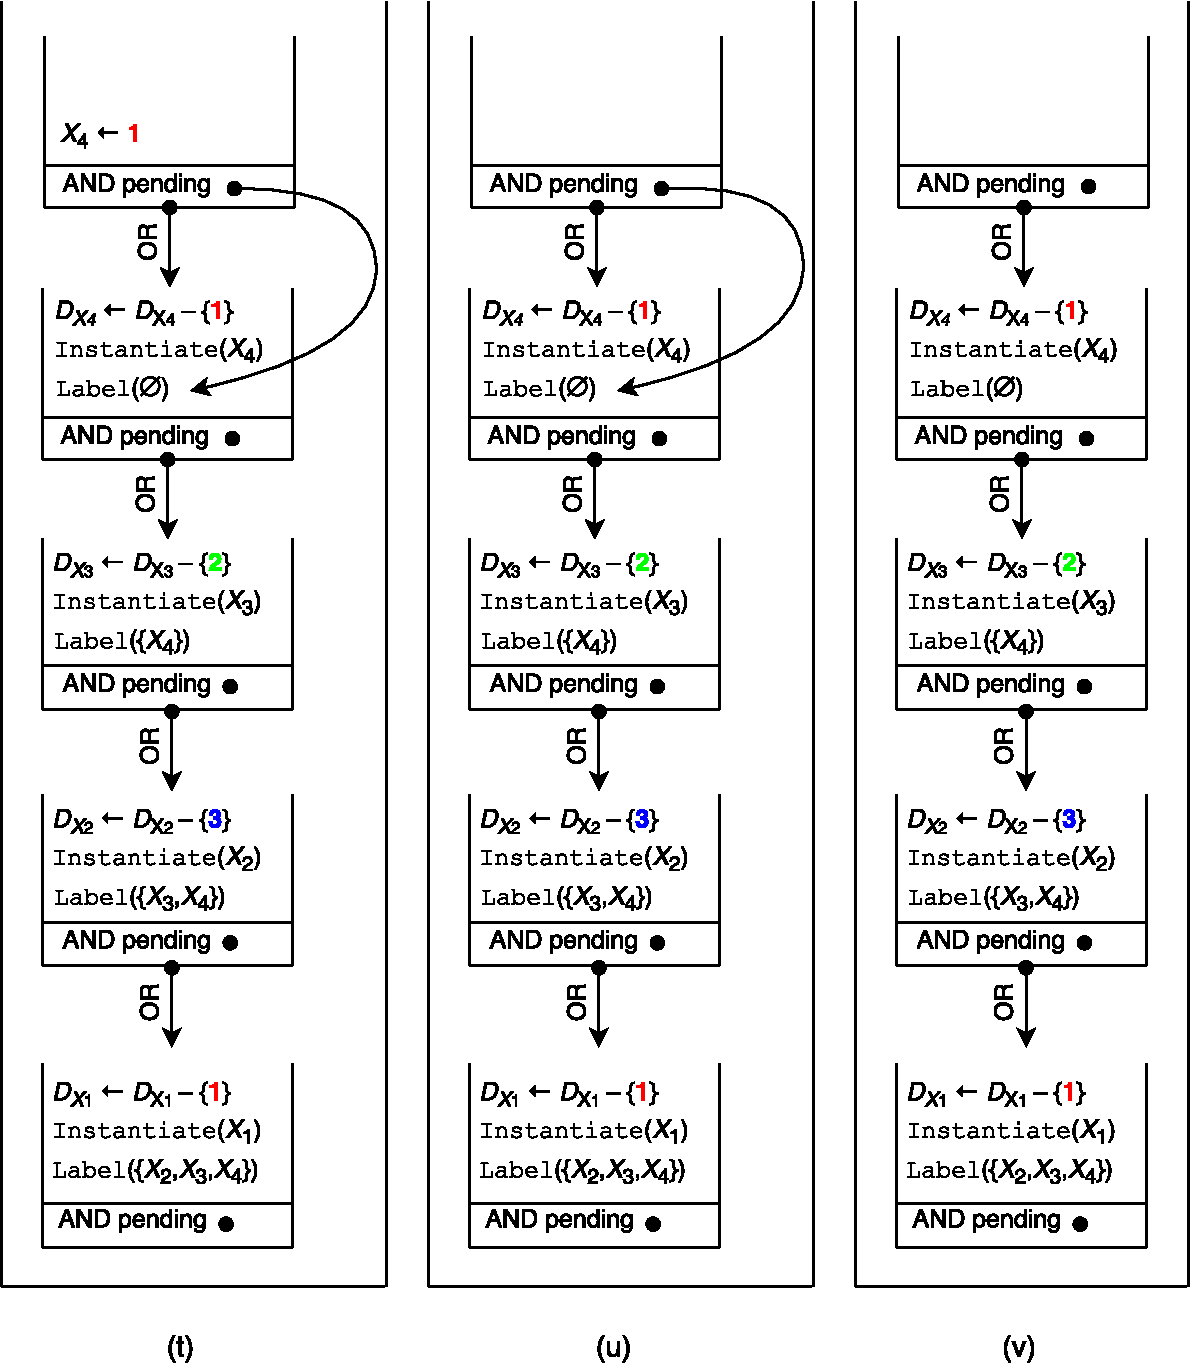
\includegraphics[width=0.9\textwidth]{figures/stacks/tuv}
  \caption{\textsc{Solve} with DFS example: $X_4$
           instantiation\label{tuv}}
\end{figure}

  \item[(f)] \texttt{Instantiate}($X_2$) is executed. As in
             (c), this is an \textsc{OR} goal, and a new
             stack is pushed.
  \item[(g)] $X_2 \! \gets \! \textcolor{red}{1}$ gets
             executed.
  \item[(h)] The assignment makes
             \textsc{PropagateConstraints} fail, as it
             violates the $X_1 \neq X_2$ constraint.
             Backtracking, i.e. popping the whole top stack,
             is activated.
  \item[(i)] $D_{X_2} \!\! \gets \!\! D_{X_2} \! - \!
             \{\textcolor{red}{1}\}$ is successfuly
             executed. This removes the ``no-good'' value.
  \item[(j)] \texttt{Instantiate}($X_2$) is executed again.
             However, this time the corresponding domain
             $D_{X_2}$ does not contain the removed value
             $\textcolor{red}{1}$. Thus, the only value left
             to assign to $X_2$ is $\textcolor{blue}{3}$.
  \item[(k)] $X_2 \! \gets \! \textcolor{blue}{3}$ is
             successfully executed.
  \item[(l)] Top stack is empty, so we fetch the ``pending''
             goal \texttt{Label}($\{X_3, X_4\}$) and set
             ``pending'' equal to ``null.'' The
             \texttt{Label} goal returns an \textsf{AND}
             goal. Its two subgoals are pushed on the top
             stack.
  \item[(m)] \texttt{Instantiate}($X_3$) returns an
             \textsf{OR} goal. When this is executed,
             another stack is pushed on top of the others.
  \item[(n)] $X_3 \! \gets \! \textcolor{red}{1}$ is
             executed.
  \item[(o)] \textsc{PropagateConstraints} fails, as the
             constraint $X_1 \neq X_3$ is violated. The top
             stack is immediately popped.
  \item[(p)] The no-good value is removed after $D_{X_3}
             \!\! \gets \!\! D_{X_3} \! - \!
             \{\textcolor{red}{1}\}$ execution.
  \item[(q)] \texttt{Instantiate}($X_3$) is executed again
             for the new domain.
  \item[(r)] The new assignment $X_3 \! \gets \!
             \textcolor{green}{2}$ is executed.
  \item[(s)] \textsc{PropagateConstraints} now succeeds and,
             as the top stack is empty, we proceed to the
             ``pending'' goal \texttt{Label}($\{X_4\}$).
             This generates
             \textsf{AND}(\texttt{Instantiate}($X_4$),
             \texttt{Label}($\{\}$)).
  \item[(t)] Again, \texttt{Instantiate}($X_4$) produces an
             \textsf{OR} goal which, in turn, forces
             \textsc{Solve} to push another stack on top of
             the others.
  \item[(u)] $X_4 \! \gets \! \textcolor{red}{1}$ is
             executed.
  \item[(v)] The ``pending'' \texttt{Label}($\emptyset$) is
             executed. By definition, this goal does not
             return any other goal. This means that the top
             stack is empty. And as there isn't any other
             ``pending'' goal, \textsc{Solve} has reached a
             solution and returns success!
\end{enumerate}

\clearpage


\section*{\centering Corrections and Improvements Synopsis}

First of all, as we mentioned in the Acknowledgments
section, we thank the reviewers for their insightful
comments and suggestions. The hexadecimal numbers inside the
brackets below, link to the corresponding patches that were
applied to the document's source code at
\url{https://github.com/pothitos/Search_Methods}

\newcommand{\commit}[1]{\texttt{[\href{https://github.com/pothitos/Search_Methods/commit/#1}{#1}]}}

\subsection*{Review 1}

\begin{itemize}
  \item The ``stack of stacks'' data structure along with
        the \textsc{Solve} algorithm are actually the
        \emph{implementation} of a framework
        (\emph{language}) that is capable of describing
        arbitrary search methods. In our work, the
        presentation of both the \emph{language} and its
        \emph{implementation} serves two objectives.
        \begin{enumerate}
          \item To easily define and support our proposed
                search method (\textsc{PoPS}) in a following
                section, along with the several classic
                methods that it is compared to. DFS is used
                in the first examples, but the framework
                supports every mentioned search method.
          \item Most importantly, even if we suppose that
                the whole framework is obvious, its
                architecture serves the separation of the
                CSP definition phase to the search method
                definition phase, which still remains the
                key goal in Constraint
                Programming\cite{Freuder2014} and has to be
                documented. Even if the ``stack of stacks''
                is implemented in many paradigms, this
                doesn't mean that every implementation is
                modular, extensible, documented, and
                independent of the CSPs that are solved.
          \end{enumerate}
  \item We made a more thorough presentation of
        Example~\ref{heuristics-pie}~\commit{379c}. In order
        to stress what lies between total randomness and
        total determinism, we added
        Example~\ref{heuristics-pie2} too~\commit{bcf8}.
  \item At least in the conducted experiments, the solution
        cost is lowered when the heuristics are \emph{not}
        blindly preferred, but for intermediate
        $\mathsf{conf}$-idence values~\commit{e4a5}.
  \item The employed heuristics in the experiments were made
        more explicit~\commit{abdf}.
  \item The specific $\mathsf{conf}$-idence values that were
        used each time are visible in the respective axes
        of the figures.
\end{itemize}

\subsection*{Review 2}

\begin{itemize}
  \item We summarized the contributions of the paper at the
        end of the Introduction~\commit{0258}.
  \item We mentioned the purpose of our hybrid heuristics at
        the end of their section, in order to link them to
        the search process where they are actually
        exploited~\commit{b4a1}. The confidence in the
        heuristics usually increases in deeper search tree
        nodes, but this is not guaranteed
        theoretically~\commit{5682}.
  \item We enriched Example~\ref{heuristics-pie} with more
        details about the heuristics' pie~\commit{379c}. We
        added one more example after this~\commit{bcf8}.
  \item The pure algorithmic part of
        Section~\ref{search-framework} was moved to the
        Appendix. Nevertheless, we kept the search method
        framework demonstration and figures in their initial
        position, to support the \textsc{PopsSample}
        illustration that follows.
\end{itemize}

\subsection*{Review 3}

\begin{enumerate}
  \item The textbook \emph{Artificial Intelligence: A Modern
        Approach} has been cited~\commit{9149}. Following
        this textbook, we explicitly described the local
        variables of our algorithms~\commit{4666}.
  \item Constrained optimization has been briefly
        introduced~\commit{212f}.
  \item We outlined the relation of distributed search
        methods to our framework and cited the related
        work~\commit{b671}.
  \item Another research direction for the next years has
        been added~\commit{48e0}.
\end{enumerate}

\subsection*{Review 4}

\begin{enumerate}
  \item Title has been changed to reflect the paper's
        relation to \textsc{Naxos Solver}~\commit{6d3a}.
  \item Typo fixed~\commit{ea7d}.
  \item Except for characterizing the indicative problems of
        the first paragraph as CSPs, we also described them
        as COPs~\commit{d7ea}. We added, later on,
        Section~\ref{COP} to formally describe constrained
        optimization. After each problem, there is a cited
        paper that describes how it can be defined as a
        CSP\slash COP.
  \item We explicitly mentioned \textsc{Naxos Solver} in the
        second paragraph and we also created a dedicated
        paragraph in the Introduction~\commit{3e23}.
        Nevertheless, as we explain in that paragraph, in
        this work we don't compare \textsc{Naxos} to the
        many existing other solvers, but we use it as the
        first \emph{environment} to host our contributions.
  \item As the list of related paradigms to the mentioned
        CSPs is too long, we stated some indicative ones for
        course scheduling~\commit{69d9}.
  \item A paragraph of contents was added~\commit{96a1}.
  \item Other solvers do solve a correctly defined CSP. We
        made a small rephrasing to be more clear with
        this~\commit{474e}.
  \item All the (sub)sections consist of at least two
        paragraphs. Some sections, e.g.\ 
        Section~\ref{preliminaries}, begin with few lines,
        indeed. However, these sections do not end with
        these few lines; these few lines just introduce the
        subsection that follows.
  \item We replaced the word ``transparent'' with
        ``extensible,'' as Gecode belongs to open source
        software. However, we noted that while other solvers
        have integrated search methods, our proposed search
        methods' framework supports defining custom search
        methods which are decoupled from our
        solver~\commit{a75a}.
  \item The reference exists, but it was cited one sentence
        later, so we moved it to the previous
        sentence~\commit{feae}.
  \item As proposed, we converted the two propositions into
        properties, as they derive from another property
        too~\commit{748e}.
  \item We explained briefly what the $\mathsf{Choices}$ set
        may contain and linked to the related definition and
        example~\commit{791b}. We also addressed negative
        heuristic values~\commit{a842}.
  \item Regarding our heuristic distribution function, we
        replaced ``gently scales randomness'' with the more
        neutral ``gradually scales
        randomness''~\commit{f1ef}.
  \item For sure, the repetition of the experiments using
        another Constraint Programming solver would have
        been yet another evidence for the efficiency of our
        proposed methods. However, the purpose of the paper
        is not to compare \textsc{Naxos} solver with the
        other solvers. Our purpose is to compare our
        proposed search methods to the classic search
        methods.

        Therefore, we selected \textsc{Naxos} as the
        \emph{environment} to conduct our experiments.
        Again, it would have been better to use other
        environments\slash solvers too. But the other
        mentioned solvers are mainly designed to facilitate
        the declaration of CSPs, not the definition of new
        search methods. (And here comes the other
        contribution of our paper, regarding the easy
        definition of new search methods in our Constraint
        Programming framework.)
\end{enumerate}

\end{document}
